\section{Framework Components}

\subsection{Introduction}

Golem Framework defines the structure of the application and the general mechanism of its operation
and provides a set of components, libraries, protocols, operations, functions, methods to perform specific tasks.
The default configuration of the framework guarantees the minimal usability of the Golem system.
The framework components allow for generic extension with new protocols and libraries.
Existing basic protocols allow for adding new operations based on existing functions and methods.
The framework can be extended with new components without disturbing its internal structure.

The individual components of the framework are described in this chapter

\subsection{Golem Node}

\subsubsection{Golem Service Bus}

Golem Service Bus is based on three basic components (Please see Figure ~\ref{fig:GSB} on page ~\pageref{fig:GSB}):

\begin{enumerate}

\item GSB API Gateway allows you to bind and unbind services on the bus via the REST GSB API

\item GSB Router is the central unit for client-client (service-service) communication, which sends messages (requests and responses) between them.

\item GSB Console allows you to manage services.

\end{enumerate}

\begin{figure}[H]
    \centering
    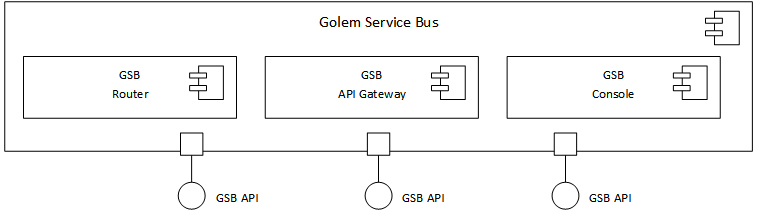
\includegraphics[width=12cm,angle=0]{./diag/Reference/GSBConcept-Reference.png}
	\caption{Golem Service Bus}
    \label{fig:GSB}
\end{figure}

Binding a service is possible via a WebSocket, Unix Socket, TCP/IP Socket endpoint or HTTP long polling.
The endpoints allow you to listen for incoming messages (requests).
The router, which uses the attached address (ex. URI identifiers), routes the path to the endpoint.
The pattern for transmitting messages between endpoints is the Routed RPC protocol.
(Please see Figure ~\ref{fig:GSBS} on page ~\pageref{fig:GSBS})

\begin{figure}[H]
    \centering
    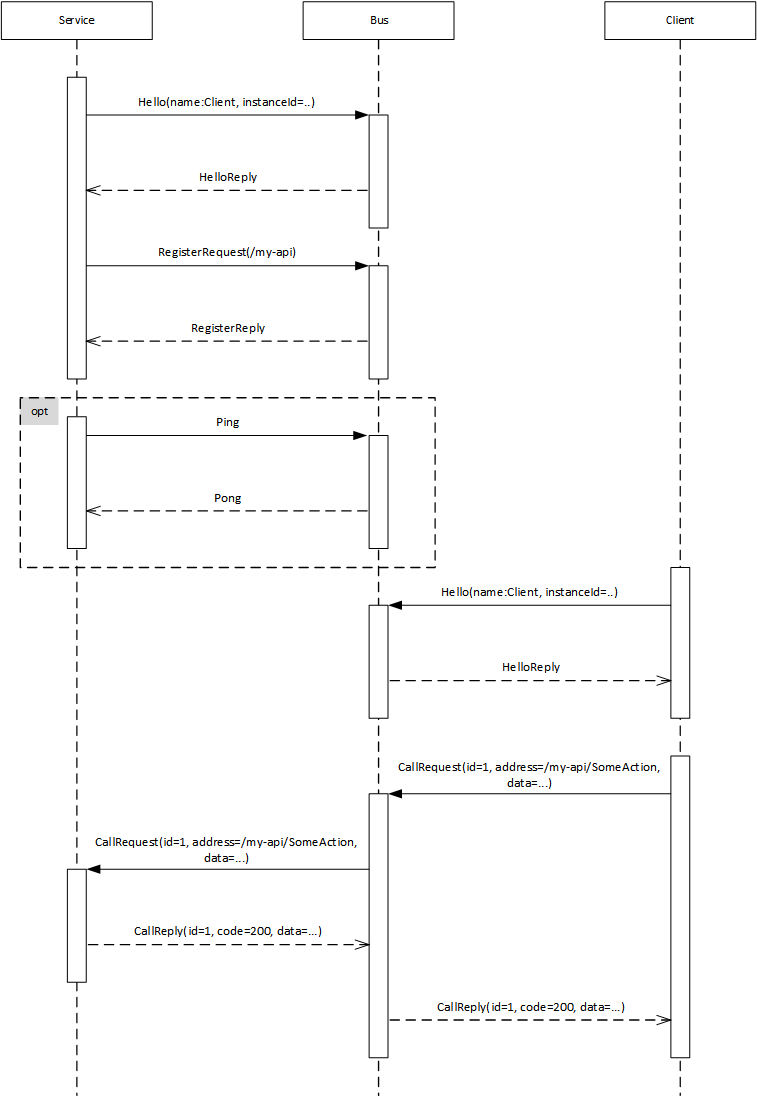
\includegraphics[width=12cm,angle=0]{./diag/Sequence/GSBCommunication-B-Sequence.png}
	\caption{GSB Communication}
    \label{fig:GSBS}
\end{figure}


\subsubsection{Golem Services}

\subsubsubsection{Golem Net Service}

In a single node, the above services communicate with each other via the Golem Service Bus (GSB).
In turn, communication between nodes takes place via the Golem Net Service (GNS) service, which provides Peer2Peer (P2P) protocols.
%This service also provides communication to the Registry and Discovery Service located on the Golem Central Net Server (GCNS).
(Please see Figure ~\ref{fig:CCR} on page ~\pageref{fig:CCR}).

\begin{figure}[H]
    \centering
    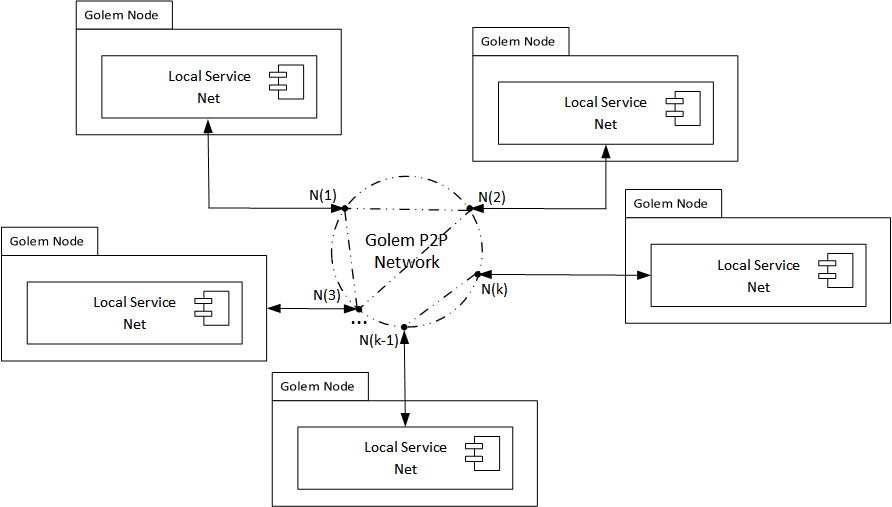
\includegraphics[width=14cm,angle=0]{./diag/Reference/CommunicationConcept-Reference.png}
	\caption{Intra and Inter Communication between Services in Nodes}
    \label{fig:CCR}
\end{figure}


In a single node, the above services communicate with each other via the Golem Service Bus (GSB), the so-called Intra Connection.
In turn, communication between nodes takes place via the Golem Net Service (GNS), which provides Peer2Peer (P2P) protocols, the so-called Inter Connection.
Golem Net Service provides the following communication models

\begin{enumerate}

\item Model Mrk0: CentraNet Proxy

\begin{enumerate}

\item Assumptions

\begin{itemize}

\item Ease of implementation
\item Must be able to penetrate Firewall above
\item Does not have to be efficient
\item Does not have to be decentralized
\item Does not have to support End2End pinging

\end{itemize}

\item Limitation

\item Flow

(Please see Figure ~\ref{fig:MM0C} on page ~\pageref{fig:MM0C}).

\begin{figure}[H]
    \centering
    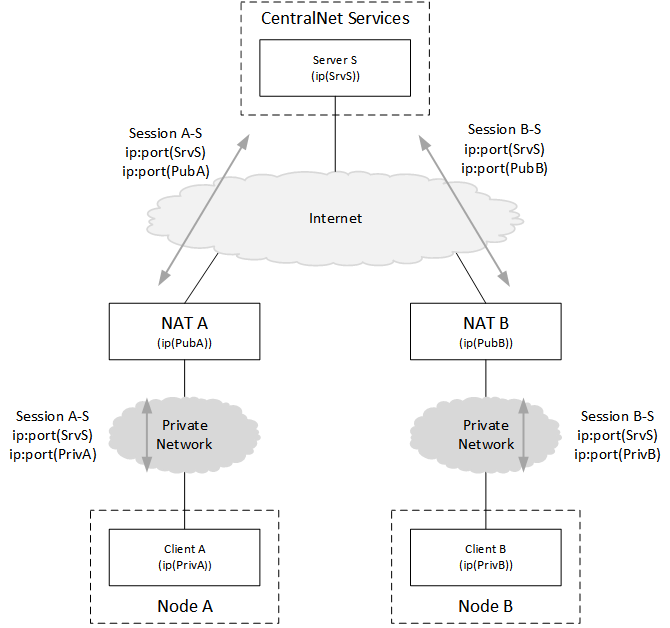
\includegraphics[width=7cm,angle=0]{./diag/Issue/Net-Mk0-1-Issue.png}
	\caption{Model Mrk0 Communication}
    \label{fig:MM0C}
\end{figure}

\begin{figure}[H]
    \centering
    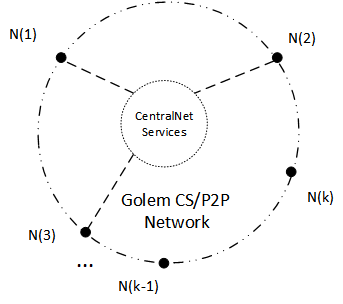
\includegraphics[width=5cm,angle=0]{./diag/Issue/Net-Mk0-2-Issue.png}
	\caption{Model Mrk0 Communication}
    \label{fig:MM0C}
\end{figure}



\item Stack

\item Sequence Diagram

\end{enumerate}

\item Model Mrk1: P2P Hybrid

Hybrid P2P networks combine elements of decentralized and centralized architectures.
The CentralNet server plays the role of managing node registration and discovery.
Hybrid P2P networks aim to achieve a balance between decentralization and efficiency.

\begin{enumerate}

\item Assumptions

\begin{itemize}

\item CentralNet Server with registration and discovery nodes service.

\item ability to send small amount of data to other nodes, about 300 kb per minute

\item if a node has a publicly available tcp/udp port, it can ask other nodes to connect,
using the ability to send data through the central server.

\item if nodes do not have publicly available tcp/udp port they can use central net to coordinate NAT hole punching
If nodes does not have publicly available tcp / udp port they can use central net to coordinate NAT hole punching

\item discovery service accepts unencrypted UDP/TCP communication.

\item in the distant future websocket / https://webrtc.rs/ - for browser compatibility.

\end{itemize} 

\item Limitation 

\item Flow

TODO Description

(Please see Figure ~\ref{fig:MM1C} on page ~\pageref{fig:MM1C}).

\begin{figure}[H]
    \centering
    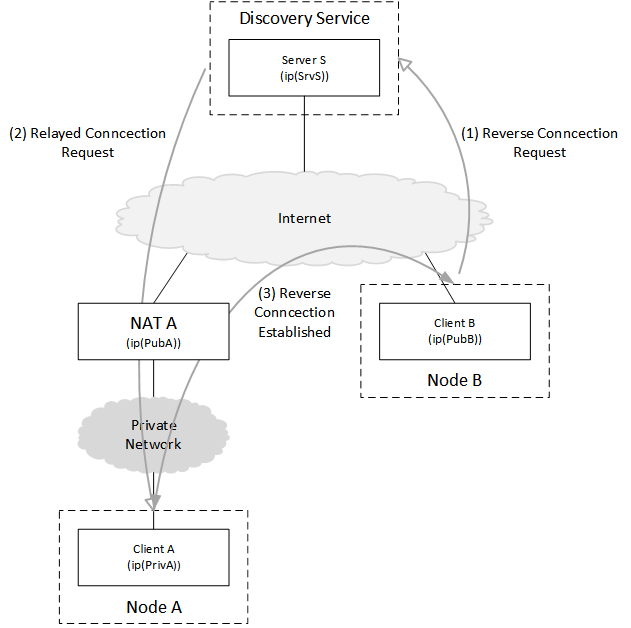
\includegraphics[width=7cm,angle=0]{./diag/Issue/Net-Mk1-1-Issue.png}
	\caption{Model Mrk1 Communication}
    \label{fig:MM1C}
\end{figure}

\begin{figure}[H]
    \centering
    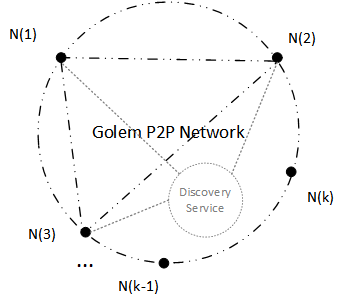
\includegraphics[width=5cm,angle=0]{./diag/Issue/Net-Mk1-2-Issue.png}
	\caption{Model Mrk1 Communication}
    \label{fig:MM1C}
\end{figure}




\item Stack

TODO Description

(Please see Figure ~\ref{fig:M1PL} on page ~\pageref{fig:M1PL}).

\begin{figure}[H]
    \centering
    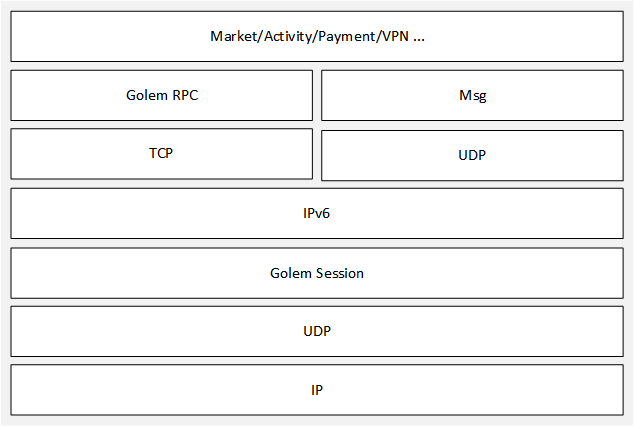
\includegraphics[width=8cm,angle=0]{./diag/Issue/NetBlock-Mk1-Issue.png}
	\caption{Protocol Mrk1 Layers}
    \label{fig:M1PL}
\end{figure}

\break

\item Sequence Diagram

TODO Description

(Please see Figure ~\ref{fig:M1SN} on page ~\pageref{fig:M1SN}).

\begin{figure}[H]
    \centering
    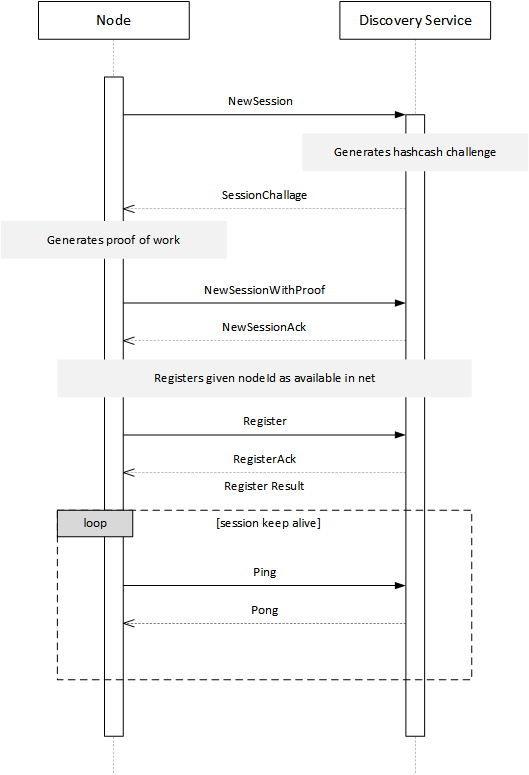
\includegraphics[width=8cm,angle=0]{./diag/Issue/SessionNegotiation-Mk1-Issue.png}
	\caption{Mrk1 Session Negotiation}
    \label{fig:M1SN}
\end{figure}


\end{enumerate} 

\item Model Mrk2: WebRTC 

\begin{enumerate} 
\item Assumptions 
\item Limitation 
\item Flow
\item Stack
\item Sequence Diagram
\end{enumerate} 

\end{enumerate}

In the Golem system, in the Net service, tuples are used to describe objects such as:
node, connection, network, status, address . (Please see Figure ~\ref{fig:NF1} on page ~\pageref{fig:NF1})

TODO figure soon

\begin{enumerate}

\item Node Objects

\begin{enumerate}

\item Object Description

TODO !!

\item Object Fields

\begin{table}[H]
\footnotesize
\begin{center}
\begin{tabular}{|p{3cm}|l|p{3cm}|p{3cm}|p{4cm}|} 
\hline
\rowcolor{lightgray}	Name	& MO.	& Type	& Example & 	Description \\
\hline

id 	& M & string & 		& Node Identifier \\
\hline 		

ip & M & string  & 		& IP address \\
\hline

\end{tabular}
\end{center}
\end{table}

\item Object State

Stateless object

\end{enumerate}

\item Connection Object

\begin{enumerate}

\item Object Description

TODO !!

\item Object Fields

\begin{table}[H]
\footnotesize
\begin{center}
\begin{tabular}{|p{3cm}|l|p{3cm}|p{3cm}|p{4cm}|} 
\hline
\rowcolor{lightgray}	Name	& MO.	& Type	& Example & 	Description \\
\hline

protocol 		& M & integer & 11		&  \\
\hline 		

localIp 		& M & string  & 0.0.0.0	& Local IP address v4 or v6 \\
\hline

localPort 		& M & integer & 1234	& Local Port \\
\hline 

remoteIp 		& M & string  & 0.0.0.0	& Local IP address v4 or v6 \\
\hline

remotePort 		& M & integer & 4321	& Local Port \\
\hline 

\end{tabular}
\end{center}

\end{table}

\item Object State

Stateless object

\end{enumerate}


\end{enumerate}

\break

\subsubsubsection{Golem Market Service}

This service has functions for creating a market of distributed computing resources.
This service allows sellers (Providers) to describe the subject of sale in the form of an offer
and buyers (Requestors) to describe the subject of demand in the form of a Demand.

In addition, the service allows for decentralized searches of offers and demands in order to associate them
based on the conditions described in offers and demands. Matched objects are represented as
proposal. An accepted and confirmed proposal allows for the creation of an agreement object, which
after being signed by the parties is a confirmation of the sale and purchase of goods such as computing resources.

(Please see Figure ~\ref{fig:MSCC} on page ~\pageref{fig:MSCC})

\begin{figure}[H]
    \centering
    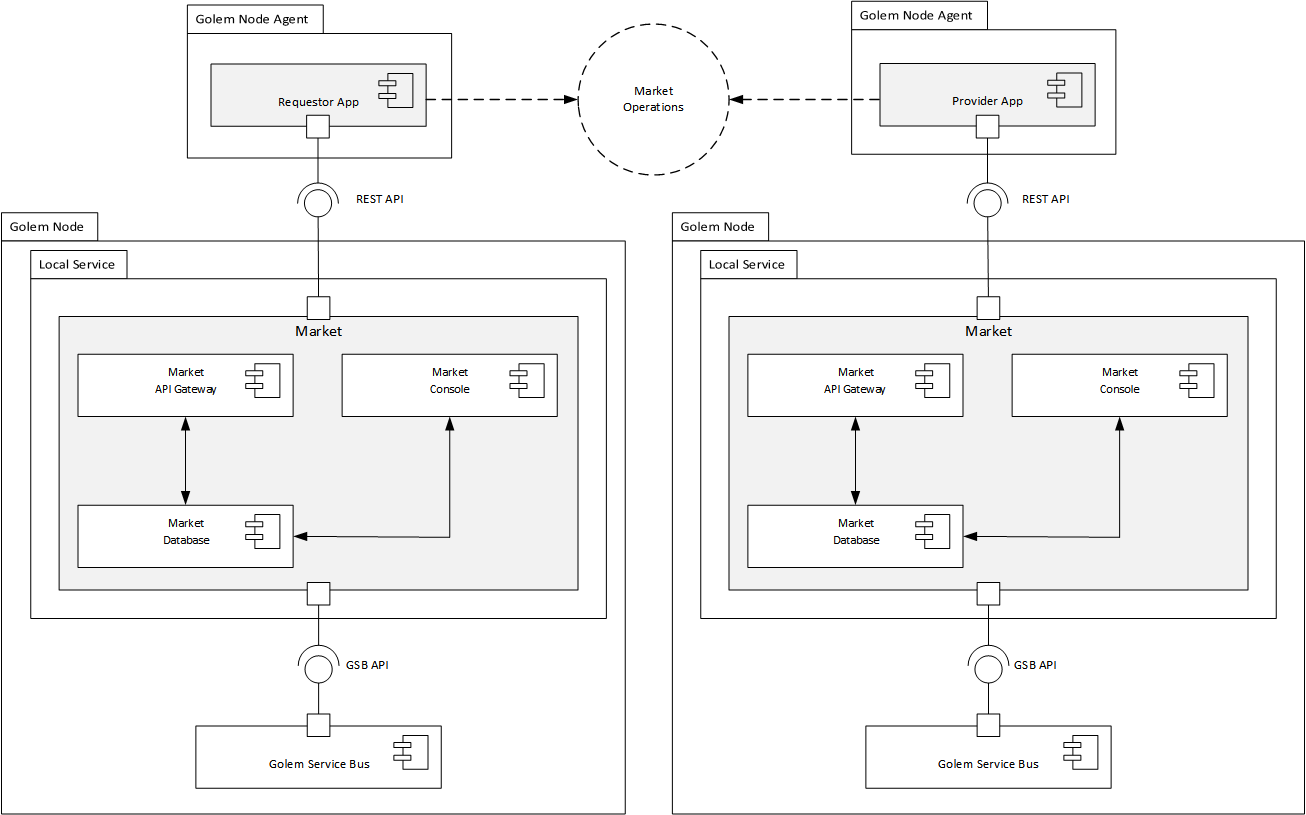
\includegraphics[width=12cm,angle=0]{./diag/Reference/MarketService-Reference.png}
	\caption{Market Service Component Concept}
    \label{fig:MSCC}
\end{figure}


The Market service is based on the tuple space (Tuples Space).
A tuple is a finite list of elements that can be used to represent a data item or a message.

In the Golem system, in the Market service, tuples are used to describe objects such as:
offer, demand, proposal, agreement. (Please see Figure ~\ref{fig:MF1} on page ~\pageref{fig:MF1}
and Figure ~\ref{fig:MF2} on page ~\pageref{fig:MF2}).

\begin{figure}[H]
    \centering
    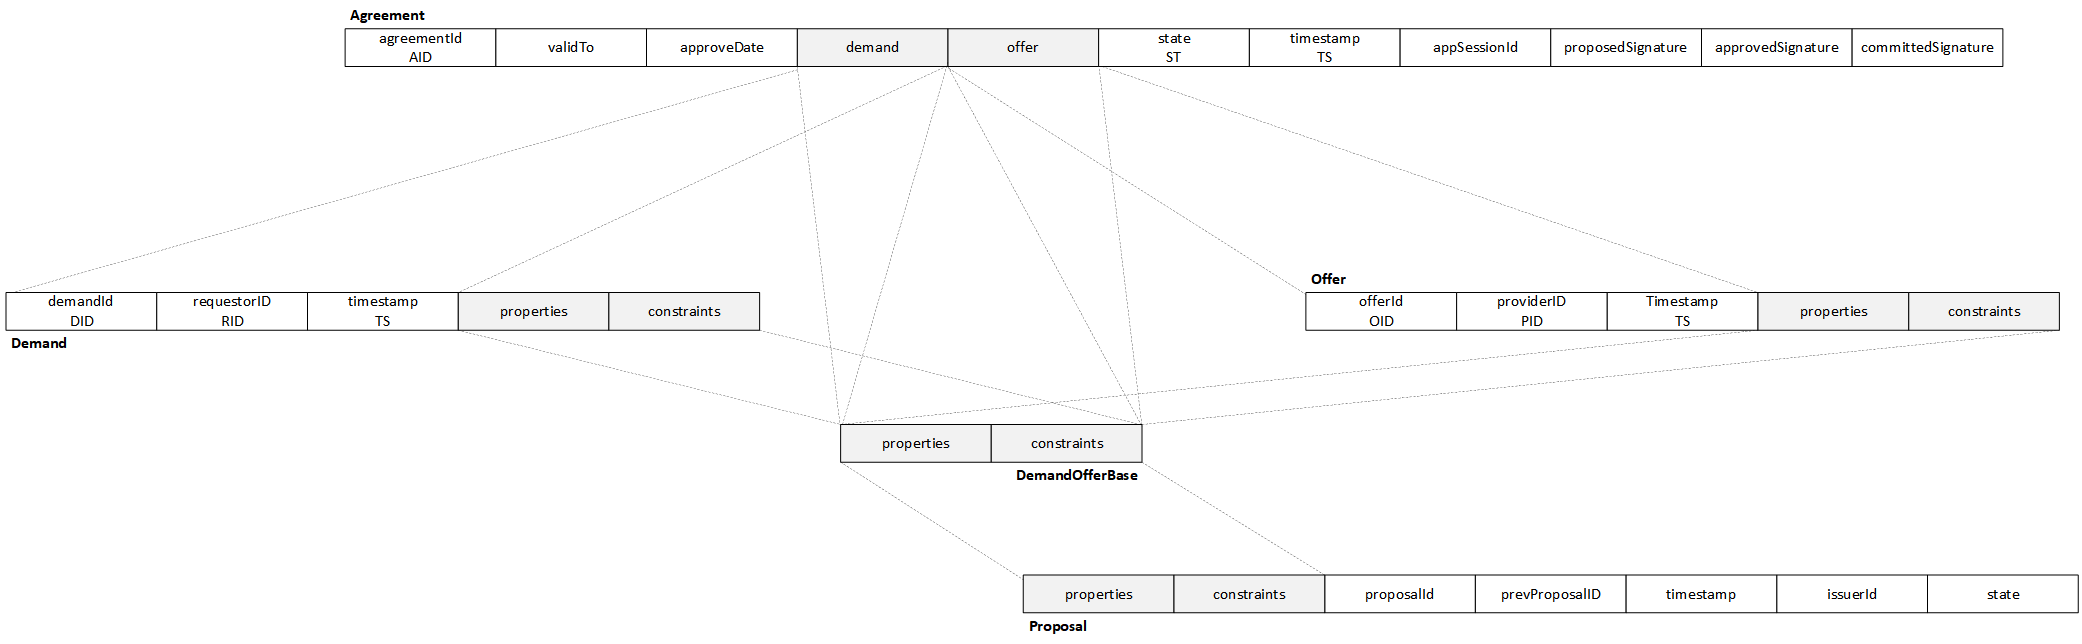
\includegraphics[width=18cm,angle=0]{./diag/Reference/MarketFrame-1-Reference.png}
	\caption{Market Objects Frame}
    \label{fig:MF1}
\end{figure}


\begin{figure}[H]
    \centering
    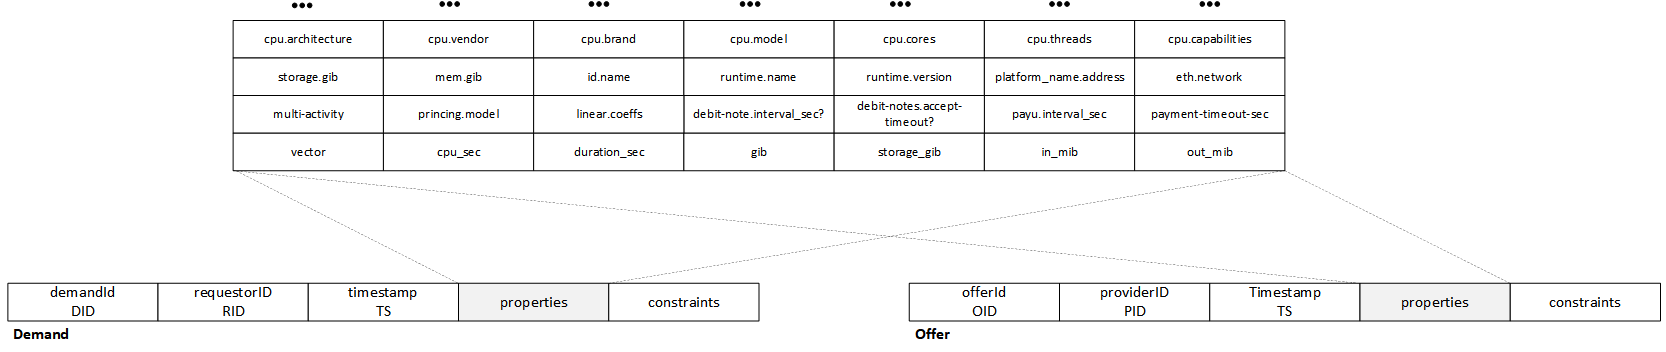
\includegraphics[width=16cm,angle=0]{./diag/Reference/MarketFrame-2-Reference.png}
	\caption{Market Objects Frame}
    \label{fig:MF2}
\end{figure}

\begin{enumerate}

\item Offer Objects

\begin{enumerate}

\item Object Description

Offer is created by Provider nodes and contains the description of the
computing resources the node has to offer, as well as any optional conditions
for their use (e.g. limiting their availability only to certain requestor nodes).

\item Object Fields

\begin{table}[H]
\footnotesize

\begin{center}
\begin{tabular}{|p{3cm}|l|p{3cm}|p{3cm}|p{4cm}|} 
\hline
\rowcolor{lightgray}	Name	& MO.	& Type	& Example & 	Description \\
\hline

offerId 	& M & string & 		& Offer Identifier \\
\hline 		

providerId & M & string  & 		& Provider Node Identifier \\
\hline

timestamp	& M	& 	string(\$date-time)	& YYYY-MM-DDThh:mm:ss.sssZ	&	Time of ???  \\
\hline

properties	& M	& 	json or flat	&		&	Offer properties \\ 
\hline

constraints	& M	& 	string	&		&	Offer constraints \\ 
\hline

\end{tabular}
\end{center}

\end{table}

\item Object State

Stateless object

\end{enumerate}

\item Demand Objects

\begin{enumerate}

\item Object Description

Demand is created by Requestor nodes and contains description of the
payload, including properties telling what capabilities the payload might
require (e.g. specific hardware architecture or features) and optionally other
conditions which ought to be satisfied by the provider nodes (e.g. asking only
for nodes which are located within specific country). 

%	Most of the content of the Demand is opaque for the Golem network

\item Object Fields

\begin{table}[H]
\footnotesize

\begin{center}
\begin{tabular}{|p{3cm}|l|p{3cm}|p{3cm}|p{4cm}|} 
\hline
\rowcolor{lightgray}	Name	& MO.	& Type	& Example & 	Description \\
\hline

demandId 	& M & string  & 		& Demand Identifier \\
\hline 		

requestorId & M & string  & 		& Requestor Node Identifier \\
\hline

timestamp	& M	& 	string(\$date-time)	& YYYY-MM-DDThh:mm:ss.sssZ	&	Time of ???  \\
\hline

properties	& M	& 	json or flat	&		&	Demand properties \\ 
\hline

constraints	& M	& 	string	&		&	Demand constraints \\ 
\hline

\end{tabular}
\end{center}
\end{table}

\item Object State

Stateless object

\end{enumerate}

\item Proposal Objects

\begin{enumerate}

\item Object Description

A proposal (Proposal object) is a Demand-Offer pair (DemandOfferBase object), with a proposalId identifier and status
and a set of field elements that allow handling of the Negotiation operation. These are: the identifier of the node submitting the proposal,
the time the proposal was created, the identifier of the proposal from the other side, to which this proposal responds.

\item Object Fields

\begin{table}[H]
\footnotesize

\begin{center}
\begin{tabular}{|p{3cm}|l|p{3cm}|p{3cm}|p{4cm}|} 
\hline
\rowcolor{lightgray}	Name	& MO.	& Type	& Example & 	Description \\
\hline

properties		& M	& 	json or flat		&												&	Proposal properties \\ 
\hline

constraints		& M	& 	string				&												&	Proposal constraints \\ 
\hline

proposalId		& M & 	string  			& 												& 	Proposal Identifier \\
\hline

issuerId		& M & 	string				&												& 	Issuer Node Identifier 	\\ 
\hline

state			& M & 	string(enum) 		& [Initial, Draft, Rejected, Accepted, Expired]	&  Proposal State	\\
\hline

timestamp		& M	& 	string(\$date-time)	& YYYY-MM-DDThh:mm:ss.sssZ						&	Time of ???  \\
\hline

prevProposalId 	& O & 	string				&												& 	Id of the Proposal from other side which this proposal responds to \\
\hline

\end{tabular}
\end{center}
\end{table}

\item Object State

(Please see Figure ~\ref{fig:PSD} on page ~\pageref{fig:PSD}).

\begin{figure}[H]
    \centering
    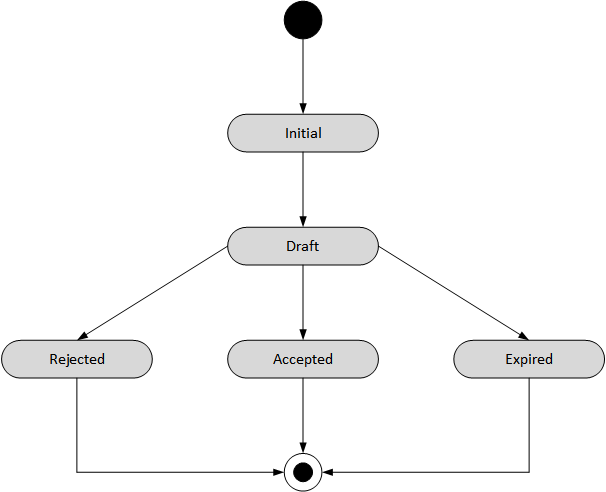
\includegraphics[width=7cm,angle=0]{./diag/Reference/ProposalState-Reference.png}
	\caption{Proposal State Diagram}
    \label{fig:PSD}
\end{figure}

\begin{table}[H]
\footnotesize

\begin{center}
\begin{tabular}{|p{3cm}|p{11cm}|} 
\hline
\rowcolor{lightgray}	State	& 	Description \\
\hline

Initial 	&	proposal arrived from the market as response to subscription \\
\hline
Draft 		&	bespoke counter-proposal issued by one party directly to other party (negotiation phase) \\
\hline
Rejected 	&	reject by other party \\
\hline
Accepted 	&	promoted into the Agreement draft \\
\hline
Expired 	&	not accepted nor rejected before validity period \\
\hline

\end{tabular}
\end{center}
\end{table}

\end{enumerate}

\item Agreement Objects

\begin{enumerate}

\item Object Description

The Agreement object is a set of basic terms of the agreement between two parties establishing their mutual relations
in relation to the subject of the service in the market space.
The basic terms of the agreement are:

\begin{itemize}

\item Established and confirmed terms of the proposal (Proposal object) within the Negotiation operation

\item Agreement object identifier

\item Agreement object state

\item Validity date of the Agreement object circulation between the parties

\item Agreement object approval date

\item Agreement object creation date

\item Correlation/session identifier used to search for events related to the action ???

\item Proposed signature

\item Confirmed signature

\item Approved signature

\end{itemize}

\item Object Fields

\begin{table}[H]
\footnotesize

\begin{center}
\begin{tabular}{|p{3cm}|l|p{3cm}|p{3cm}|p{4cm}|} 
\hline
\rowcolor{lightgray}	Name	& MO.	& Type	& Example & 	Description \\
\hline

agreementId			& M & string 				&				& 	Agreement Identifier \\
\hline

demand				& M	& object 				&				& 	Demand		\\
\hline

offer 				& M & object 				& 				& 	Offer 		\\
\hline

validTo				& M & string(\$date-time)	& YYYY-MM-DDThh:mm:ss.sssZ & End of validity period. 
																			Agreement needs to be approved, rejected or cancelled before this date; 
																			otherwise will expire. \\
\hline

approveDate			& M & string(\$date-time)	& YYYY-MM-DDThh:mm:ss.sssZ & Agreement approval timestamp \\
\hline

state 				& M & string(enum) 				&[Proposal, Pending, Cancelled, Rejected, Approved, Expired, Terminated] & Agreement State \\
\hline

timestamp			& M	& 	string(\$date-time)	& YYYY-MM-DDThh:mm:ss.sssZ	&	Time of ???  \\
\hline

appSessionId		& O &	string 				&							& 	A correlation/session identifier used for querying events related to an action 
																				where this appSessionId has been specified		\\
\hline

proposedSignature 	& O & 	string 				&							&			\\
\hline

approvedSignature 	& O & 	string 				& 							&			\\
\hline

committedSignature	& O &	string 				& 							& 			\\
\hline

\end{tabular}
\end{center}
\end{table}

\item Object State

(Please see Figure ~\ref{fig:ASD} on page ~\pageref{fig:ASD}).

\begin{figure}[H]
    \centering
    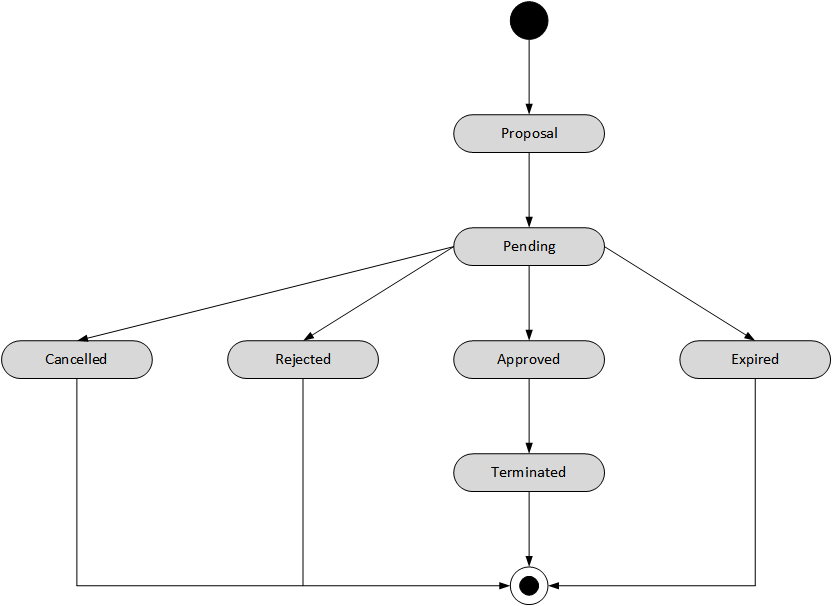
\includegraphics[width=9cm,angle=0]{./diag/Reference/AgreementState-Reference.png}
	\caption{Agreement State Diagram}
    \label{fig:ASD}
\end{figure}

\begin{table}[H]
\footnotesize

\begin{center}
\begin{tabular}{|p{3cm}|p{11cm}|} 
\hline
\rowcolor{lightgray}	State	& 	Description \\
\hline

Proposal	&	newly created by a Requestor (draft based on Proposal) \\
\hline
Pending		&	confirmed by a Requestor and send to Provider for approval \\
\hline
Cancelled 	& 	by a Requestor \\
\hline
Rejected 	&	by a Provider \\
\hline
Approved 	&	by both sides \\
\hline
Expired 	&	not approved, rejected nor cancelled within validity period \\
\hline
Terminated 	&	finished after approval. \\
\hline

\end{tabular}
\end{center}
\end{table}

\end{enumerate}

\item DemandOfferBase Object

\begin{enumerate}

\item Object Description

The DemandOfferBase object is a temporary object that collects negotiated terms related to the service item.

\item Object Fields

\begin{table}[H]
\footnotesize

\begin{center}
\begin{tabular}{|p{3cm}|l|p{3cm}|p{3cm}|p{4cm}|} 
\hline
\rowcolor{lightgray}	Name	& MO.	& Type	& Example & 	Description \\
\hline

properties	& M	& 	json or flat	&		&  Temporary Proposal properties \\ 

\hline

constraints	& M	& 	string	&		&	Temporary Proposal constraints \\ 

\hline

\end{tabular}
\end{center}
\end{table}

\item Object State

Stateless object

\end{enumerate}

\end{enumerate}

\break

The Market Space is used to define interaction operations on these objects such as:

\begin{enumerate}
\item  Observation Operation

\begin{enumerate}

\item Description

The Market Observation operation is implemented by a set of Scan functions. 
These functions, together with REST API methods, allow to aggregate data from currently circulating 
offers (Offer object) and demands (Demand object).

The BeginScan() function initiates the scanning operation by accepting the filtering criteria and 
returning scanId. The results are aggregated and collected by the CollectScanResults() function.
The EndScan() function closes the data aggregation process.

The criteria for searching the Golem network market are defined using the service model description language (Golem SMDL),
where the filter syntax is based on the LDAP filter syntax. Depending on the needs, simple or complex search criteria can be defined.

(Please see Figure ~\ref{fig:MOO} on page ~\pageref{fig:MOO}).

\item Sequence Diagram

\begin{figure}[H]
    \centering
    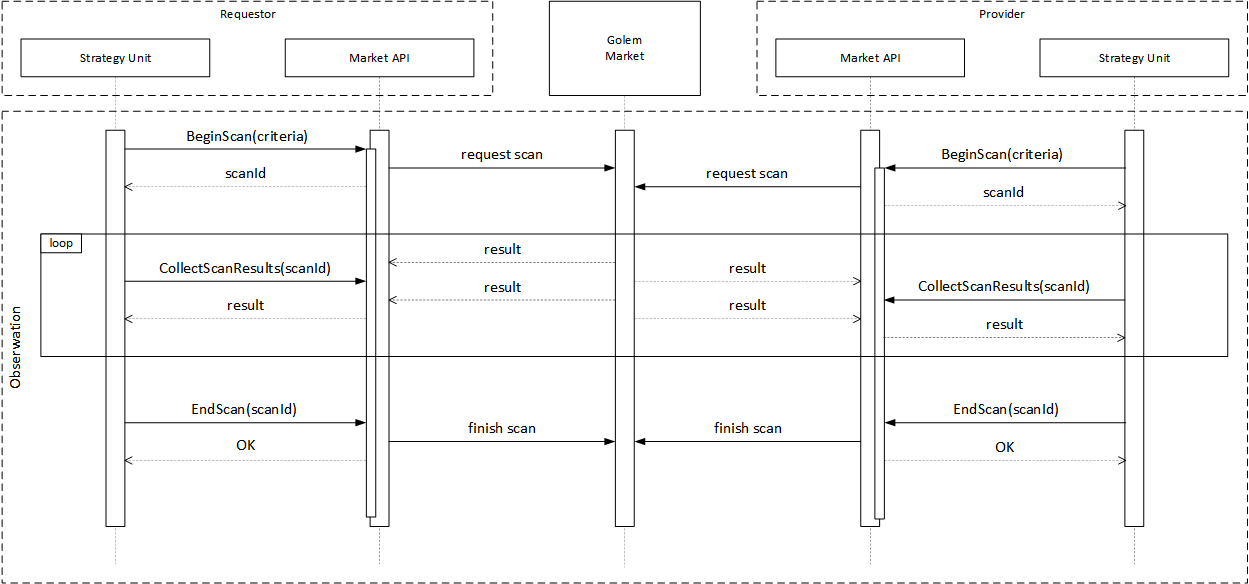
\includegraphics[width=14cm,angle=0]{./diag/Sequence/MarketObservation-B-Sequence.png}
	\caption{Market Observation Operation}
    \label{fig:MOO}
\end{figure}

\item Functions and Methods

\begin{table}[H]
\footnotesize

\begin{center}
\begin{tabular}{|p{3cm}|p{7cm}|p{1.5cm}|p{4cm}|} 
\hline
\rowcolor{lightgray}	Function Name	& API Method Name	& 	Side	&	Description \\
\hline

BeginScan 				& POST /scan								&	Both	&	\\
\hline

CollectScanResult		& GET /scan/\{subscriptionId\}/events		&	Both 	& ?? subscriptionId or scanId ??	\\
\hline

EndScan 				& DELETE /scan/\{subscriptionId\}/events	&	Both 	& ?? subscriptionId or scanId ??	\\
\hline

\end{tabular}
\end{center}
\end{table}

\end{enumerate}

\item  Discovery Operation

\begin{enumerate}

\item Description

The Discovery operation is implemented by a set of Subscribe functions. These functions, together with REST API methods, 
allow for the aggregation of data from currently circulating active offers (Offer object) and active demands (Demand object).

The Subscribe() function publishes the offer (Offer object) and demand (Demand object) on the Golem Network Market, respectively.
The aggregated results in the form of proposals (Proposal object) with matching Demand-Offer pairs are collected by the Collect() function.
The Unsubscribe() function disables the availability of offers and demands on the Golem Network Market.

The Discovery operation is the only one that involves indirect communication (e.g. via a P2P network).
The subsequent phases are direct (one-to-one)

(Please see Figure ~\ref{fig:MDO} on page ~\pageref{fig:MDO}).

\item Sequence Diagram

\begin{figure}[H]
    \centering
    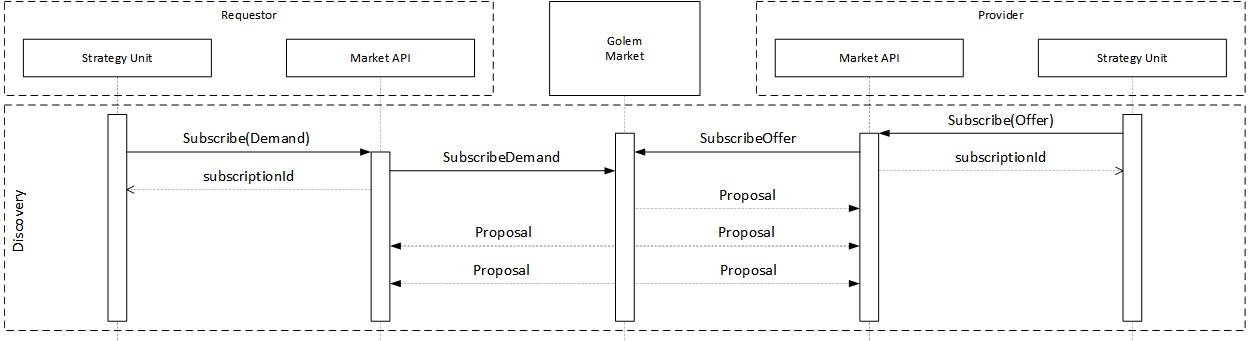
\includegraphics[width=14cm,angle=0]{./diag/Sequence/MarketDiscovery-B-Sequence.png}
	\caption{Market Discovery Operation}
    \label{fig:MDO}
\end{figure}

\item Functions and Methods

\begin{table}[H]
\footnotesize

\begin{center}
\begin{tabular}{|p{3cm}|p{7cm}|p{1.5cm}|p{4cm}|} 
\hline
\rowcolor{lightgray}	Function Name	& API Method Name	& 	Side	&	Description \\
\hline

Subscribe			&	POST /offers							&	Provider	&	Publishes Provider capabilities via Offer \\
\hline

Subscribe			&	POST /demands							& 	Requestor	&	Publishes Requestor capabilities via Demand \\
\hline

Unsubscribe			&	DELETE	/offers/\{subscriptionId\}		&	Provider	&	Stop subscription for published Offer \\
\hline

Unsubscribe			&	DELETE	/demands/\{subscriptionId\}		&	Requestor	&	Stop subscription for published Demand \\
\hline	 

CollectDemands ?	&	GET	/offers/\{subscriptionId\}/events	&	Provider &	Reads Market responses to published Offer \\
\hline

CollectOffers ?		&	GET	/demands/\{subscriptionId\}/events	&	Requestor &	Reads Market responses to published Demand \\
\hline

Collect				& 	POST /offers/\{subscriptionId\}/ \newline propertyQuery/\{queryId\} & Provider & Handles dynamic property query \\
\hline

Collect				& 	POST /demands/\{subscriptionId\}/ \newline propertyQuery/\{queryId\} & Requestor & Handles dynamic property query \\
\hline 

					&	GET /offers								&	Provider	&	Fetches all active Offers which have been published by the Provider \\
\hline

					&	GET /demands							& 	Requestor	&	Fetches all active Demands which have been published by the Requestor \\
\hline	 

\end{tabular}
\end{center}
\end{table}

\end{enumerate}

\item  Negotiation Operation

\begin{enumerate}

\item Description

The Negotiation operation is implemented by a set of REST API functions and methods that allow for reaching a consensus between the parties
by matching offers and demands. This is done by automatic or semi-automatic exchange of documents (Offer and Demand objects)
between the parties in the form of proposals (Proposal object). 
The negotiation conditions are described by the service model description language (Golem SMDL) 
where the filter syntax is based on the LDAP filter syntax.

The Collect() function collects aggregated results in the form of proposals (Proposal object) from the data contained 
in the offer (Offer object) and in the demand (Demand object).

The CounterProposal() function In the case of the Requestor node, it creates and sends a modified version of the original demand 
(Demand object as a counterproposal) adapted to the previously received Proposal (i.e. Offer).
In the case of the Provider node, it creates and sends a modified version of the original offer (the Offer object as a counterproposal) 
adapted to the previously received proposal (i.e. Demand). The function for both cases changes the state of the Proposal object to Draft 
and returns the created proposalId. 

The RejectProposal() function effectively ends the negotiation chain - it clearly indicates
that the sender will not create another counterproposal. If the negotiations reach a consensus, 
then an agreement (the Agreement object) is generated by the CreateAgreement() function of the Agreement operation. 

The Provider node retrieves the proposal (Demand) with the given proposalId using the GetProposalDemand() method. 
The Requestor node retrieves the proposal (Offer) with the given proposalId using the GetProposalOffer() method.

(Please see Figure ~\ref{fig:MNO} on page ~\pageref{fig:MNO}).

\item Sequence Diagram

\begin{figure}[H]
    \centering
    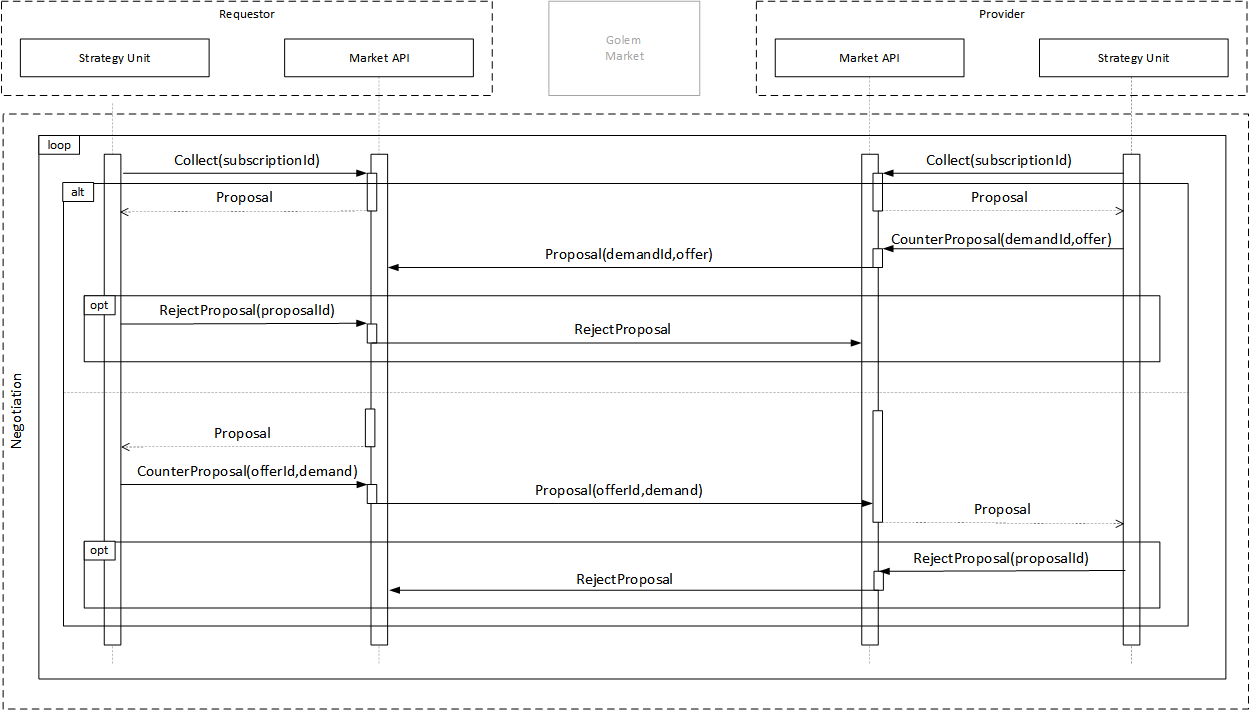
\includegraphics[width=14cm,angle=0]{./diag/Sequence/MarketNegotiation-B-Sequence.png}
	\caption{Market Negotiation Operation}
    \label{fig:MNO}
\end{figure}

\item Functions and Methods

\begin{table}[H]
\footnotesize

\begin{center}
\begin{tabular}{|p{3cm}|p{7cm}|p{1.5cm}|p{4cm}|} 
\hline
\rowcolor{lightgray}	Function Name	& API Method Name	& 	Side	&	Description \\
\hline

Collect			&	GET /offers/\{subscriptionId\}/events	&	Provider	&	Reads Market responses to published Offer \\
\hline

Collect			&	GET /demands/\{subscriptionId\}/events	&	Requestor	&	Reads Market responses to published Demand \\
\hline

CounterProposal	&	POST /offers/\{subscriptionId\}/ \newline proposals/\{proposalId\}	&	Provider	&	Responds with a bespoke Offer to received Demand \\
\hline

CounterProposal	&	POST /demands/\{subscriptionId\}/ \newline proposals/\{proposalId\}	&	Requestor	&	Responds with a bespoke Demand to received Offer \\
\hline

RejectProposal	&	POST /offers/\{subscriptionId\}/ \newline proposals/\{proposalId\}/reject & Provider & Reject Proposal Demand \\
\hline

RejectProposal	&	POST /demands/\{subscriptionId\}/ \newline proposals/\{proposalId\}/reject & Requestor & Reject Proposal Offer \\
\hline

				&	GET /offers/\{subscriptionId\}/ \newline proposals/\{proposalId\}	&	Provider	&	Fetches Proposal (Demand) witch given id \\
\hline

				&	GET /demands/\{subscriptionId\}/ \newline proposals/\{proposalId\}	&	Requestor	&	Fetches Proposal (Offer) witch given id \\
\hline

\end{tabular}
\end{center}
\end{table}

\end{enumerate}

\item  Agreement Operation

\begin{enumerate}

\item Description

The Agreement operation is implemented by a set of REST API functions and methods that allow for the finalization of the Negotiation operation by
confirming receipt of the agreement signed by both parties (Agreement object).

The CreateAgreement() function creates an agreement (Agreement object) from the negotiated proposal (Proposal object) by the Requestor node.

The agreement created by the ConfirmAgreement() function is signed with the Applicant's signR key and sent to the Provider.

The RejectAgreement() function is used to interrupt the Agreement operation by the Provider node.

Running the RejectAgreement() function interrupts the Agreement operation, giving the Requestor node the possibility of returning the negotiation operation,
which can send a new proposal (Proposal object).

The CancelAgreement() function is used to interrupt the Agreement operation by the Requestor node.

This is possible only until the Agreement is approved or rejected by the Provider and before it expires.

The WaitForApproval() function is used to set the time to prepare resources to start the calculations as part of the Activity service operation.
This function is initialized by the Requestor node for the Provider node. After the set time has elapsed, the Requestor node can
re-call this function for the same agreement identifier (agreementId).

The ApproveAgreement() function is used to approve the agreement by the Provider node. It is used when the environment with
resources on the Provider node is ready to start the calculations by the Requestor node as part of the Activity service operation.

The TerminateAgreement() function is used to terminate the agreement in the Approved state.
The other party is notified about the decision of the calling party to terminate the "current" agreement. Available for both types of nodes.

The GetTerminateReason method is used to retrieve the reason for termination of the agreement reported during the call to the TerminateAgreement() function. Available for both types of nodes.

The AgreementEvents method is used to collect events related to the agreement (the Agreement object). These are

\begin{itemize}

\item AgreementApprovedEvent : 	indicates that the Agreement has been approved by the Provider.
								The Provider is now ready to accept the request to start the Activity
								as described in the negotiated agreement.
								The corresponding Provider approveAgreement call returns Approved after emitting this event.

\item AgreementRejectedEvent : 	indicates that the Provider has called rejectAgreement, which effectively stops the Agreement negotiation.
								The Applicant can try to return to the Negotiation phase by sending a new Proposal.

\item AgreementCancelledEvent : indicates that the Applicant has called cancelAgreement, which effectively stops the Agreement negotiation.

\item AgreementTerminatedEvent : indicates that the Agreement has been terminated by the specified party (includes a signature).

\end{itemize}

The ListAgreements method is used to retrieve information about agreements. It uses optional filters:

\begin{itemize}

\item state: [Proposal, Pending, Cancelled, Rejected, Approved, Expired, Terminated ]

\item creation date and time

\item application session identifier

\end{itemize}

The GetAgreementContent() function is used to retrieve an agreement (Agreement object) based on a given identifier (agreementId).

The ValidateAgreementContent() function is used to verify an agreement (Agreement object) sent as a byte stream.

(Please see Figure ~\ref{fig:MAO} on page ~\pageref{fig:MAO}).

\item Sequence Diagram

\begin{figure}[H]
    \centering
    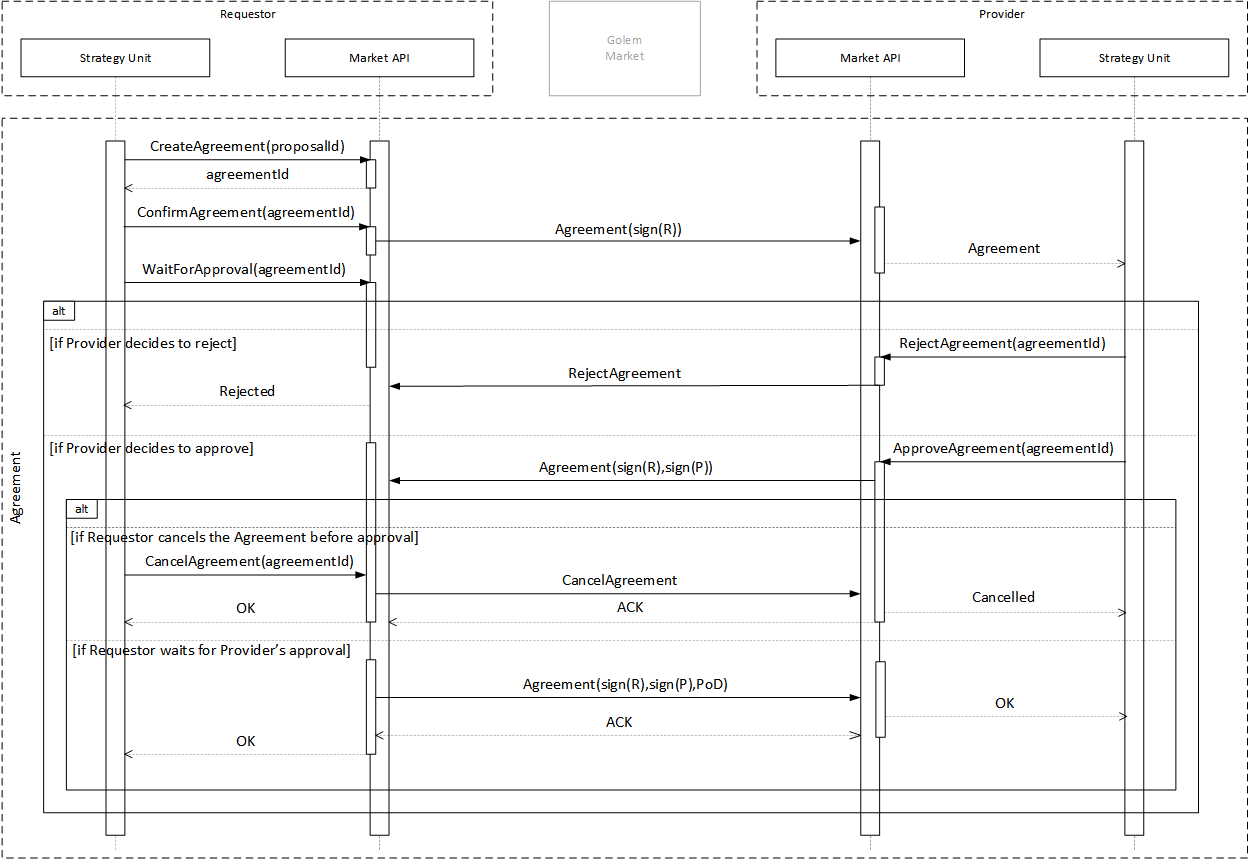
\includegraphics[width=14cm,angle=0]{./diag/Sequence/MarketAgreement-B-Sequence.png}
	\caption{Market Agreement Operation}
    \label{fig:MAO}
\end{figure}

\item Functions and Methods

\begin{table}[H]
\footnotesize

\begin{center}
\begin{tabular}{|p{3cm}|p{7cm}|p{1.5cm}|p{4cm}|} 
\hline
\rowcolor{lightgray}	Function Name	& API Method Name							& 	Side	&	Description \\
\hline

CreateAgreement		&	POST /agreements											& Requestor	&	Creates Agreement from selected Proposal \\
\hline

					&	GET /agreements												&	Both	&	List agreements with optional filters \\
\hline

GetAgreement \newline Content	&	GET /agreements/\{agreementId\}					&	Both	&	Fetches  agreement with agreement id \\
\hline

ValidateAgreement \newline Content &												&	Both	&	Offline function for validation of agreement submitted in the form of byte stream \\
\hline

ConfirmAgreement	& POST /agreements/\{agreementId\}/ \newline terminate			& Requestor & 	Sends Agreement proposal to the Provider \\
\hline

WaitForApproval		& POST /agreements/\{agreementId\}/ \newline wait				& Requestor & 	Waits for Agreement approval by the Provider \\
\hline

CancelAgreement		& POST /agreements/\{agreementId\}/ \newline cancel				& Requestor &	Cancels Agreement	\\
\hline

TerminateAgreement	& POST /agreements/\{agreementId\}/ \newline terminate			& Both		&	Terminates approved Agreement \\
\hline

					& POST /agreements/\{agreementId\}/ \newline terminate/reason 	& Both 		& 	Gets termination reason reported when terminateAgreement operation was called \\
\hline					

					& GET /agreementEvents											& Both 		& 	Collect events related to an Agreement \\
\hline

ApproveAgreement	& POST /agreements/\{agreementId\}/ \newline Approve			& Provider	&	Approves Agreement proposed by the Requestor \\
\hline

RejectAgreement		& POST /agreements/\{agreementId\}/ \newline reject				& Provider	&	Rejects Agreement proposed by the Requestor	\\
\hline

\end{tabular}
\end{center}
\end{table}

\end{enumerate}

\end{enumerate}

%\begin{enumerate}
%    \item Service Profile
%    \item Service Protocol
%    \item Service Interface
%    \item Service Workflow
%\end{enumerate}

\subsubsubsection{Golem Activity Service}

This service has tools that allow the Requestor's applications and services to be launched on the Provider's computing resources,
while simultaneously measuring the use of these resources in accordance with the concluded contract in the form of an agreement. 
The measurement of the use of resources is recorded in the form of metrics in the Usage Counters Vector (UCV) object.


(Please see Figure ~\ref{fig:ASCC} on page ~\pageref{fig:ASCC})

\begin{figure}[H]
    \centering
    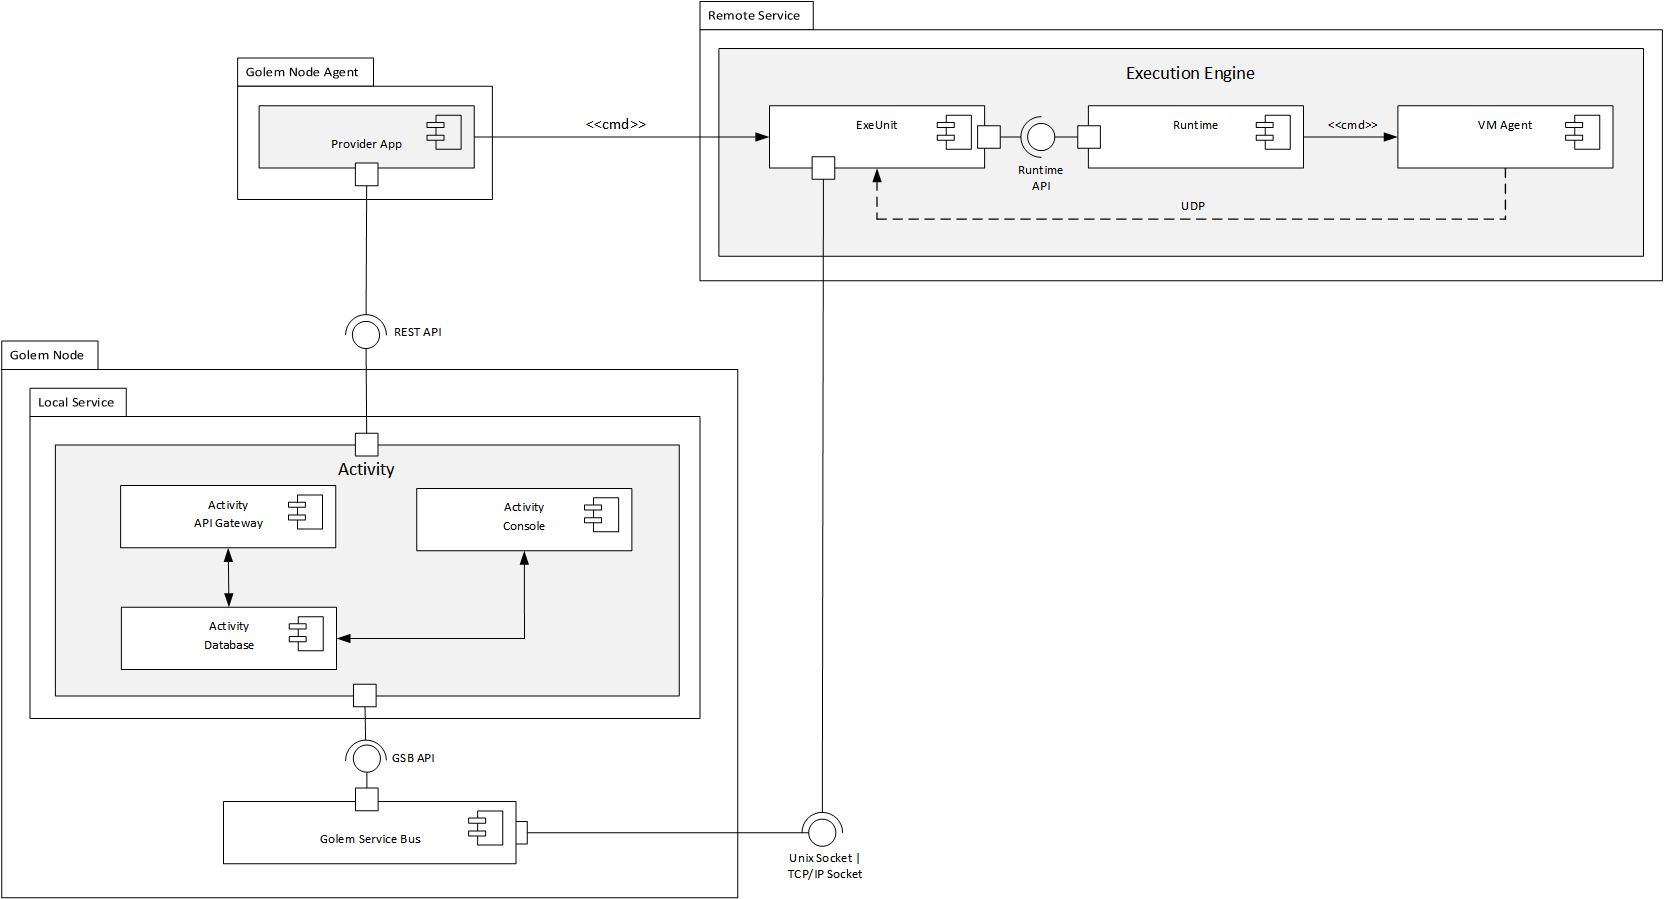
\includegraphics[width=14cm,angle=0]{./diag/Reference/ActivityService-Reference.png}
	\caption{Activity Service Component Concept}
    \label{fig:ASCC}
\end{figure}


%%%% Objects 

In the Golem system, in the Activity service, tuples are used to describe objects such as:
ActivityUsage, ADR (Activity Detail Record), ActivityState. (Please see Figure ~\ref{fig:MF1} on page ~\pageref{fig:MF1}
and Figure ~\ref{fig:MF2} on page ~\pageref{fig:MF2}).

\begin{figure}[H]
    \centering
    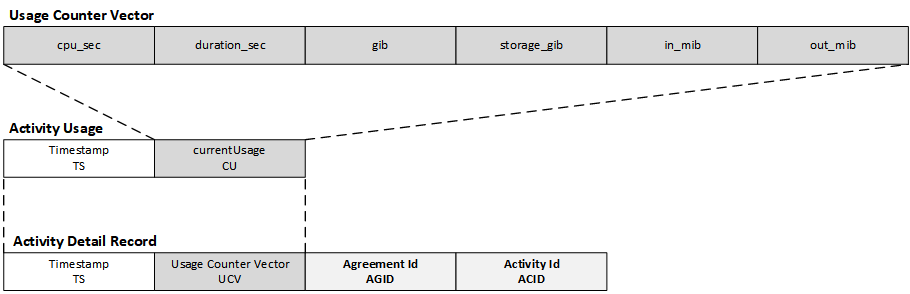
\includegraphics[width=11cm,angle=0]{./diag/Reference/ActivityFrame-1-Reference.png}
	\caption{Market Objects Frame}
    \label{fig:AF1}
\end{figure}


\begin{figure}[H]
    \centering
    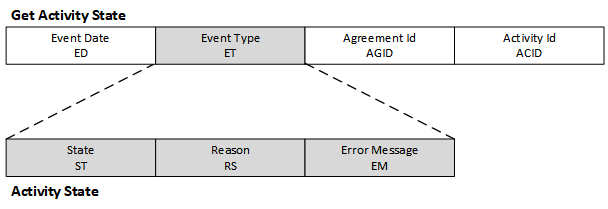
\includegraphics[width=8cm,angle=0]{./diag/Reference/ActivityFrame-2-Reference.png}
	\caption{Market Objects Frame}
    \label{fig:AF2}
\end{figure}


\begin{enumerate}

\item ActivityUsage Object

\begin{enumerate}

\item Object Description

The ActivityUsage object is created by calling GetCurrentUsage() function
and GET method /activity/\{activityId\}/usage. Queries can be called in any Activity state.

\item Object Fields

\begin{table}[H]
\footnotesize
\begin{center}
\begin{tabular}{|p{3cm}|l|p{3cm}|p{3cm}|p{4cm}|} 
\hline
\rowcolor{lightgray}	Name	& MO.& Type		& Example 	& 	Description \\
\hline

currentUsage 		&  O & number(\$double) 	& [123.5, 34000]	&  	Current vector of usage counters consumed by the Activity. 
																	The sequence of values corresponds to Usage Vector property 
																	(golem.usage.vector) as indicated in the Agreement (Offer part).\\
\hline 		

timestamp 			& M  & integer 			& 	0				& 	Usage update timestamp (UTC) \\
\hline

\end{tabular}
\end{center}
\end{table}

\item Object State

Stateless object

\end{enumerate}

\item Activity Detail Record

\begin{enumerate}

\item Object Description

The ADR object is a generic object derived from the ActivityUsage object.
The ADR object has ActivityUsage fields and Activity process identification fields (activityId) along with the Agreement process (agreementId)
This object is a proposal to consider for flexible and optimal design of settlements within the billing operation of the Payment process.
It has the properties of CDR (Call Detail Record) objects.

\item Object Fields

\begin{table}[H]
\footnotesize
\begin{center}
\begin{tabular}{|p{3cm}|l|p{3cm}|p{3cm}|p{4cm}|} 
\hline
\rowcolor{lightgray}	Name	& MO.& Type		& Example 	& 	Description \\
\hline

currentUsage 		&  O & number(\$double) 	& [123.5, 34000]	&  	Current vector of usage counters consumed by the Activity. 
																	The sequence of values corresponds to Usage Vector property 
																	(golem.usage.vector) as indicated in the Agreement (Offer part).\\
\hline 		

timestamp 			&  M &  string(\$date-time) & 	YYYY-MM-DDThh:mm:ss.sssZ	& 	Usage update timestamp (UTC) \\
\hline

agreementId 		&  M & string 			& 					& 	Agreement Identifier \\
\hline

activityId 			&  M & string 			& 					& 	Activity Identifier \\
\hline

\end{tabular}
\end{center}
\end{table}

\item Object State

Stateless object

\end{enumerate}

\item GetActivityState

TODO !!!

\item ActivityState

\begin{enumerate}

\item Object Description

The ActivityState object is created by calling GetState() function
and GET method /activity/\{activityId\}/state. This function queries the state of the Activity. 

\item Object Fields

\begin{table}[H]
\footnotesize
\begin{center}
\begin{tabular}{|p{3cm}|l|p{3cm}|p{3cm}|p{4cm}|} 
\hline
\rowcolor{lightgray}	Name	& MO.	& Type	& Example & 	Description \\
\hline

state				& M	&	string(enum)	& 	&	State pair tuple (CurrentState, NextState). 
													NextState is equal to null if there is no pending transition between states.\\
\hline  

reason 				& O	&	string			&	& 	Reason for Activity termination \\
\hline

errorMessage		& O	&	string			&	& 	If error caused state change - error message shall be provided. \\
\hline
 
\end{tabular}
\end{center}
\end{table}

\item Object State

(Please see Figure ~\ref{fig:AASD} on page ~\pageref{fig:AASD}).

\begin{figure}[H]
    \centering
    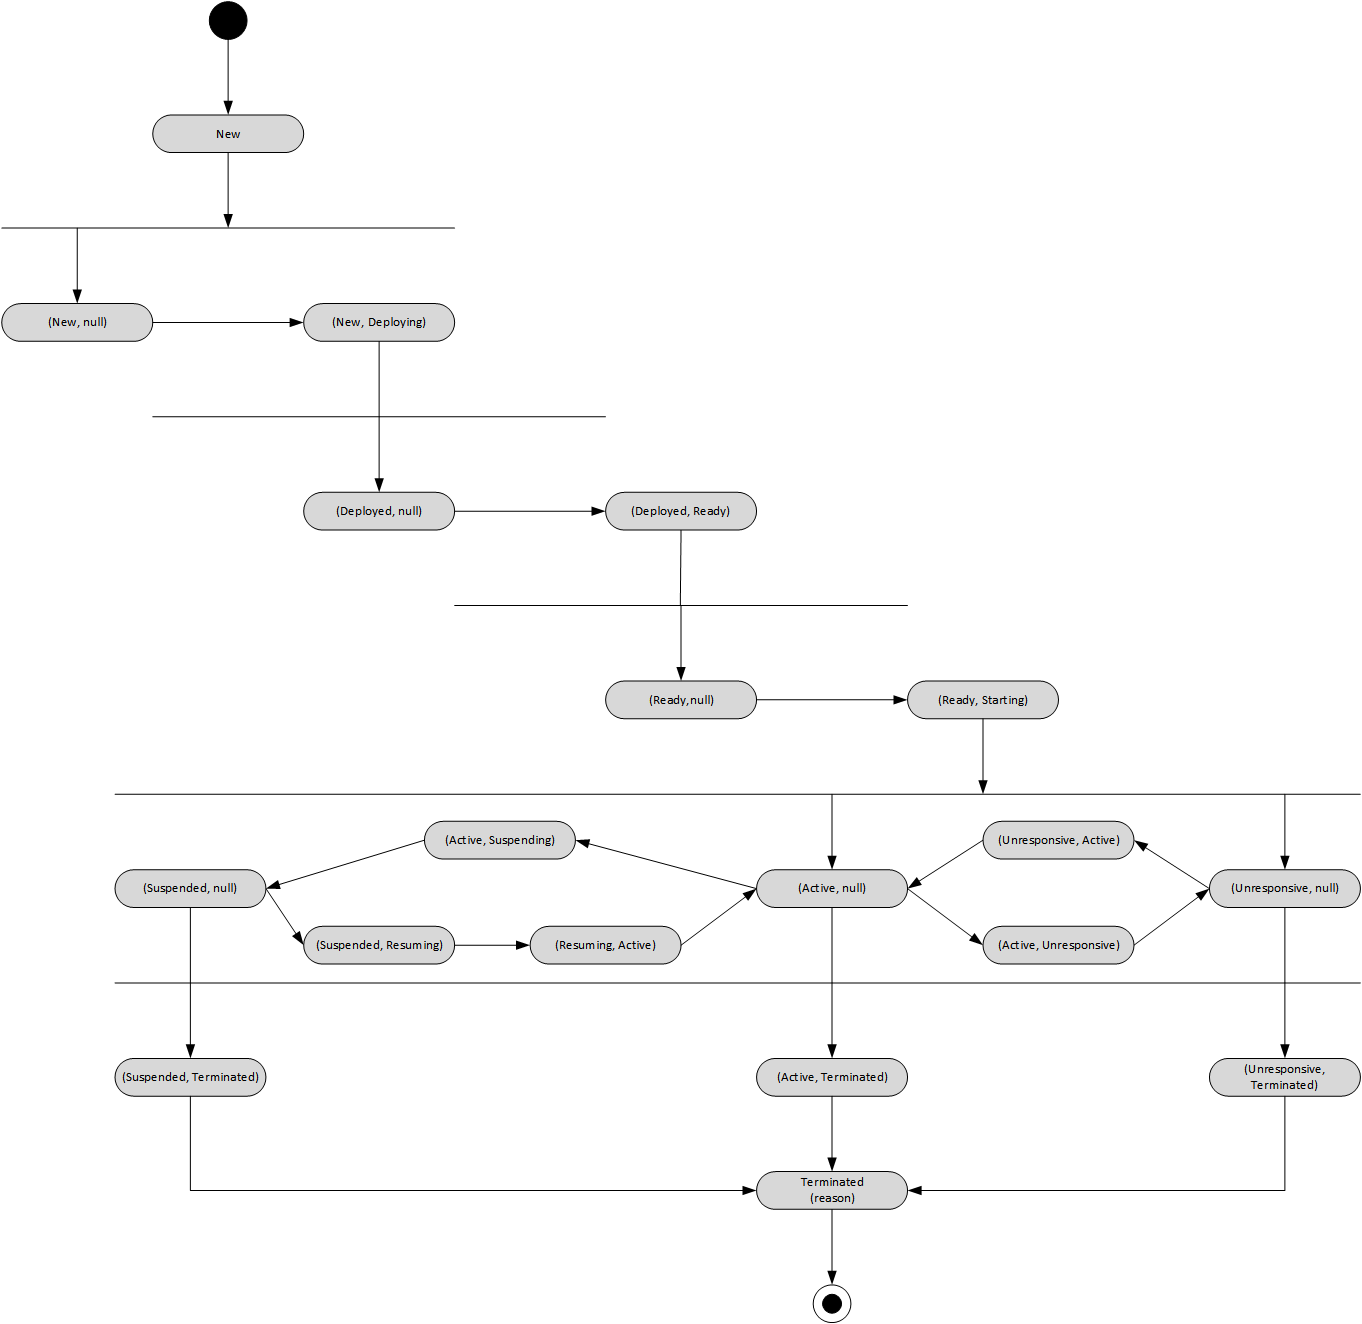
\includegraphics[width=14cm,angle=0]{./diag/Reference/ActivityState-Reference.png}
	\caption{Activity State Diagram}
    \label{fig:AASD}
\end{figure}

\begin{table}[H]
\footnotesize

\begin{center}
\begin{tabular}{|p{3cm}|p{11cm}|} 
\hline
\rowcolor{lightgray}	State	& 	Description \\
\hline

New			&	 \\
\hline
Deploying	&	? \\
\hline
Deployed 	& 	? \\
\hline
Ready 		&	 \\
\hline
Starting 	&	 \\
\hline
Active 		&	 \\
\hline
Unresponsive 	&	 \\
\hline
Suspending 	&	? \\
\hline
Sunspended 	&	? \\
\hline
Resuming 	&	 \\
\hline
Terminated 	&	 \\
\hline

\end{tabular}
\end{center}
\end{table}

\end{enumerate}

\end{enumerate}

The Activity Space is used to define interaction operations on these objects such as:

\begin{enumerate}
\item  Control Operation

\begin{enumerate}

\item Description

TODO

(Please see Figure ~\ref{fig:ACO} on page ~\pageref{fig:ACO}).

\item Sequence Diagram

\begin{figure}[H]
    \centering
    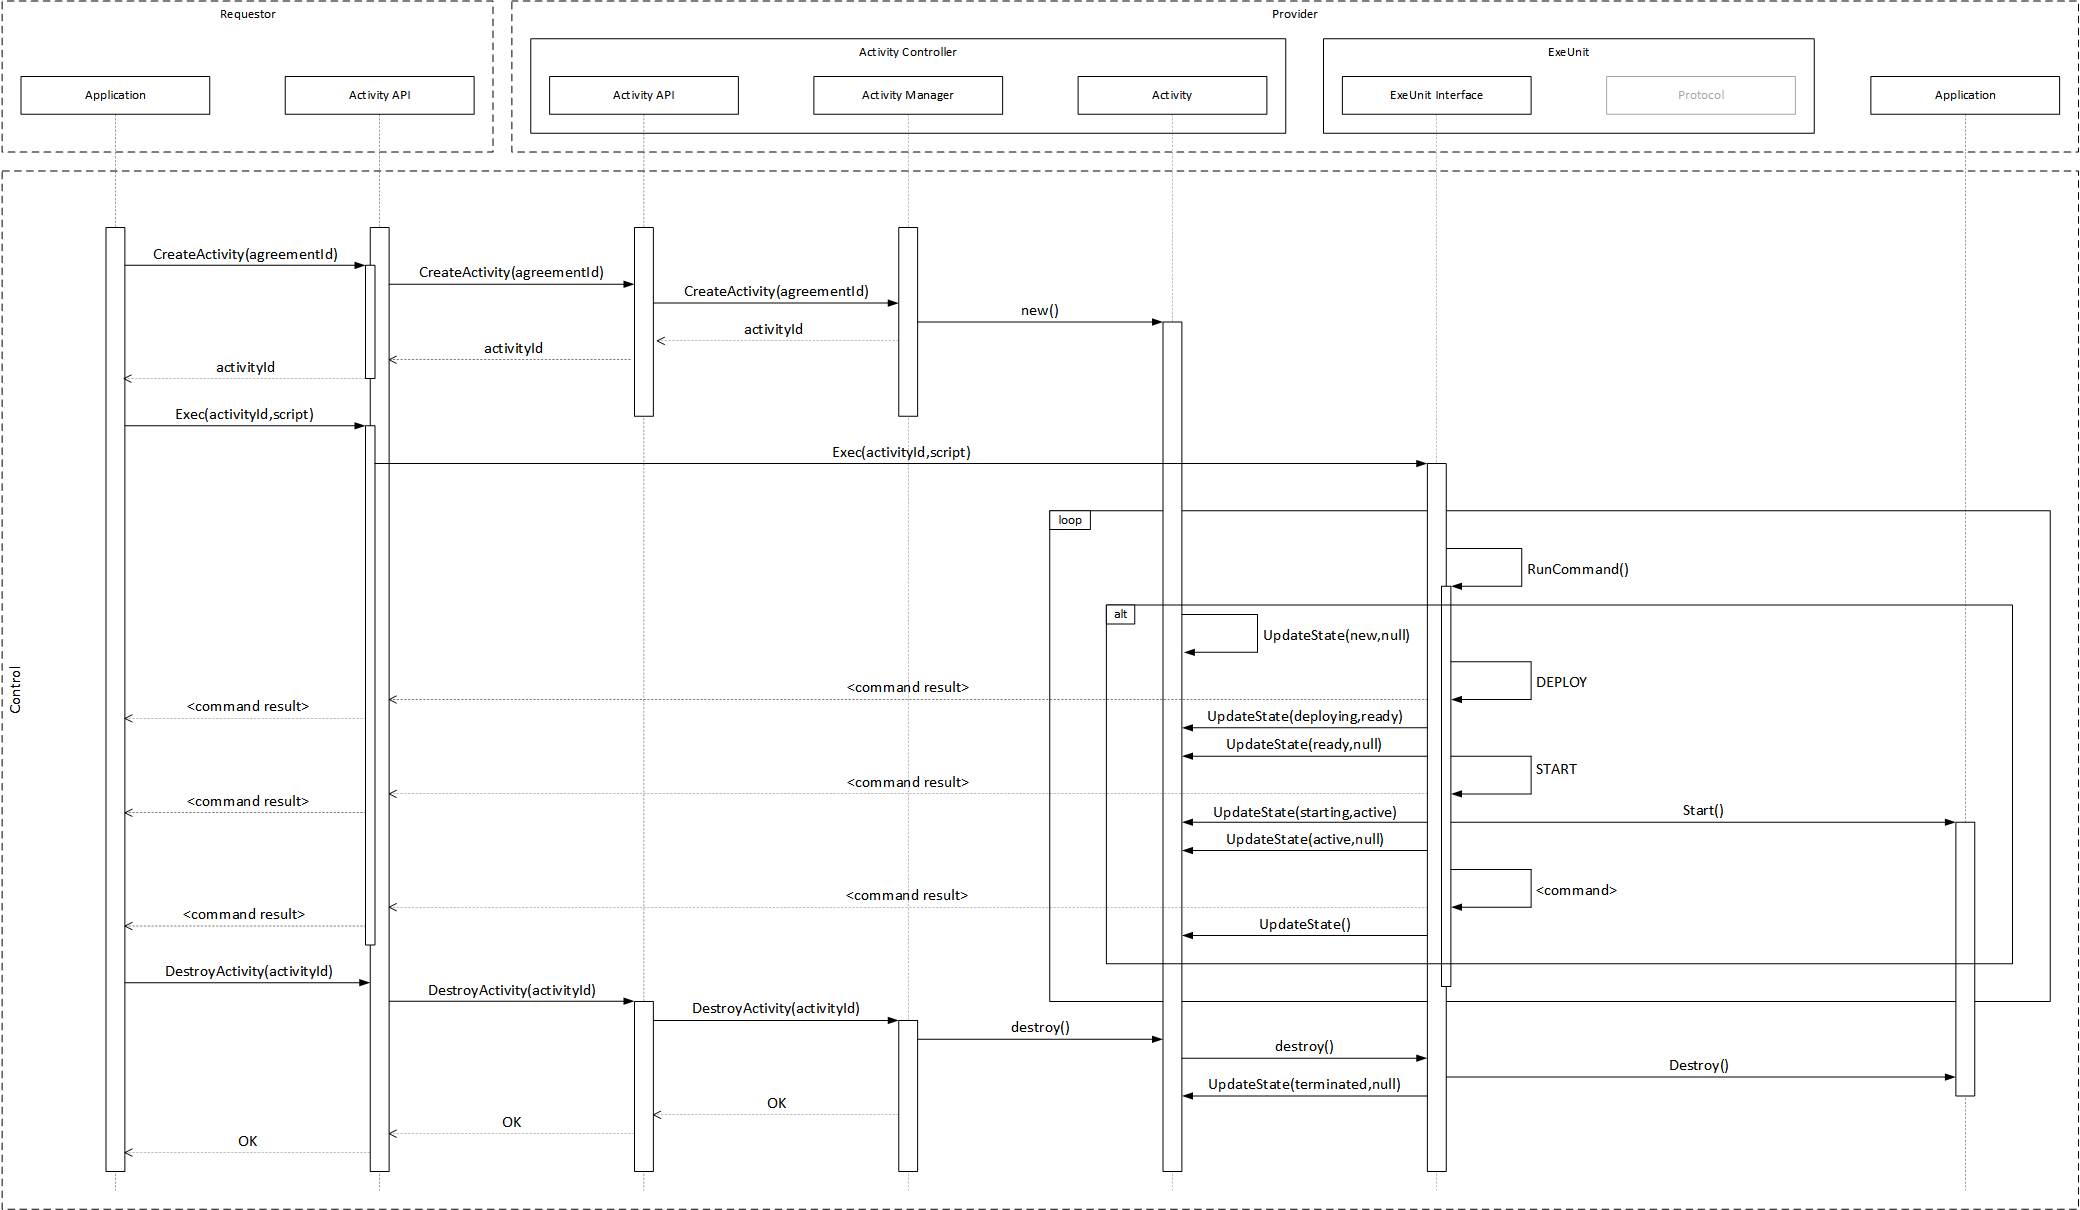
\includegraphics[width=16cm,angle=0]{./diag/Sequence/ActivityControl-B-Sequence.png}
	\caption{Activity Control Operation}
    \label{fig:ACO}
\end{figure}

\item Functions and Methods

\begin{table}[H]
\footnotesize

\begin{center}
\begin{tabular}{|p{3cm}|p{7cm}|p{1.5cm}|p{4cm}|} 
\hline
\rowcolor{lightgray}	Function Name	& API Method Name	& 	Side	&	Description \\
\hline

CreateActivity 				& POST 	/activity	&	Requestor	&  Creates new Activity based on given Agreement	\\
\hline

Exec						& POST /activity/\{activityId\}/exec	&	Requestor 	&  Executes an ExeScript batch within a given Activity	\\
\hline

GetExecBatchResults 		& GET /activity/\{activityId\}/ \newline exec/\{batchId\}	&	Both 	&  Queries for ExeScript batch result	\\
\hline

DestroyActivity				& DELETE /activity/\{activityId\}	& Requestor & Destroys given Activity \\
\hline

GetState					& GET /activity/\{activityId\}/state	& Both	& Get state of specified Activity \\
\hline

GetCurrentUsage				& GET /activity/\{activityId\}/usage	& Both & Get usage of specified Activity \\
\hline

GetRunningCommand			& GET /activity/\{activityId\}/command	& Requestor & Get running commands for specified Activity \\
\hline

ListenEvent					& GET /events	&	Provider	&	Fetch Requestor command events \\
\hline

ChangeState					& PUT /activity/\{activityId\}/state & Provider & Set state of specified Activity \\
\hline

							& GET /activity/\{activityId\}/agreement & Provider & Returns agreementId corresponding to the Activity \\
\hline

\end{tabular}
\end{center}
\end{table}

\end{enumerate}

\end{enumerate}


\subsubsubsection{Golem Payment Service}

This service enables settlements between the parties based on the terms contained in the contract. 
Usage Counters Vector (UCV) objects created in the Golem Activity Service and the settlement terms included in the agreement 
are used to settle the sale-purchase item. The Usage Counters Vector (UCV) associated with the agreement and activity creates 
Activity Detail Record (ADR) objects. Settlement functions allow the ADR object to be transformed into a Debit Note (DN) object, 
where the total incremental settlement amounts for using Provider resources are included. The frequency of creating and sending 
Debit Notes objects between the parties is included in the agreement. The state of completing the use of Provider resources allows 
for the generation of an invoice summarizing the agreement between the parties. 
Payment is made via the blockchain operator. Optimization of payment transaction costs is possible by setting the terms of this operation 
in the agreement object.

(Please see Figure ~\ref{fig:PSCC} on page ~\pageref{fig:PSCC})

\begin{figure}[H]
    \centering
    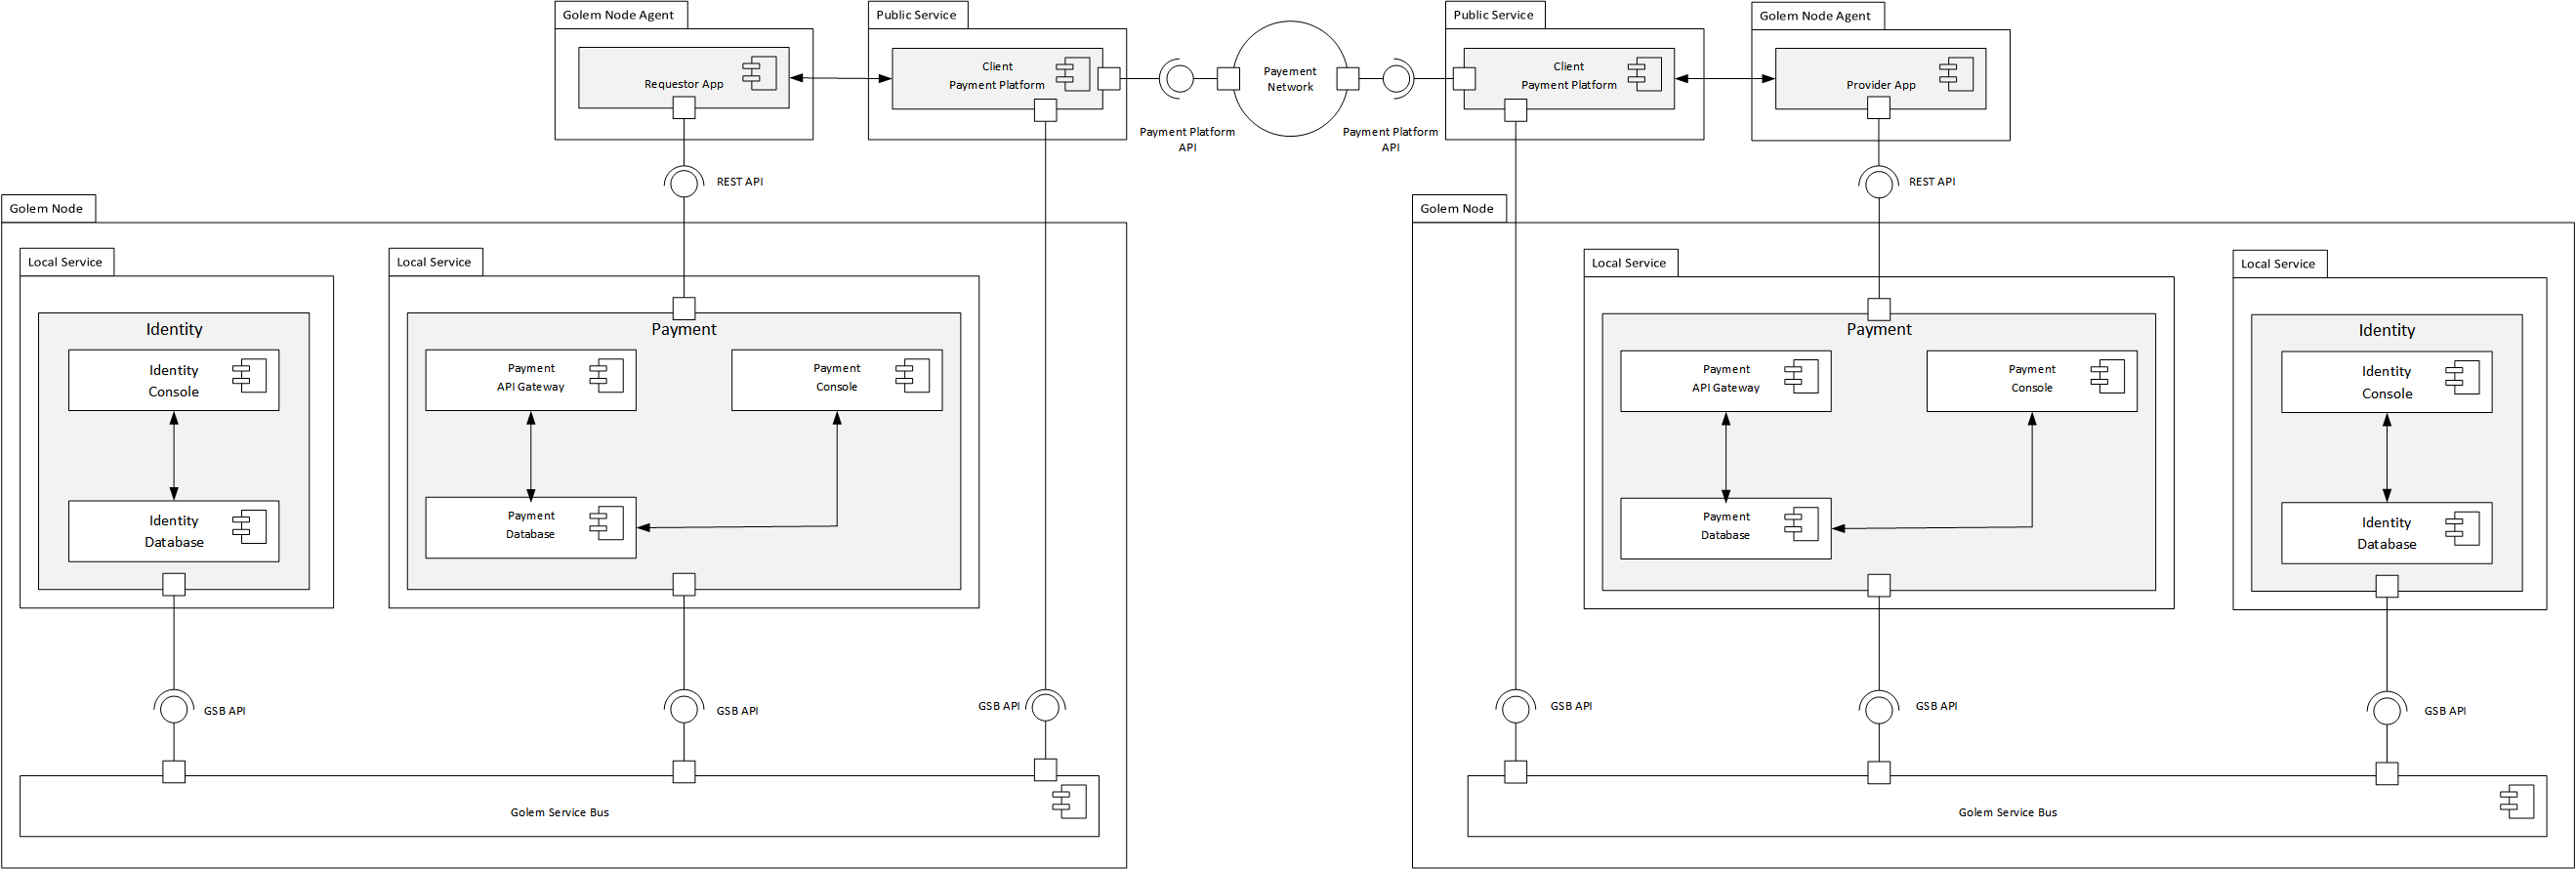
\includegraphics[width=18cm,angle=0]{./diag/Reference/PaymentService-Reference.png}
	\caption{Payment Service Component Concept}
    \label{fig:PSCC}
\end{figure}



In the Golem system, in the Payment service, tuples are used to describe objects such as:
vector usage counters, activity detail record, debit note, invoice . 
(Please see Figure ~\ref{fig:PF1} on page ~\pageref{fig:PF1} and Figure ~\ref{fig:PF2} on page ~\pageref{fig:PF2})

\begin{figure}[H]
    \centering
    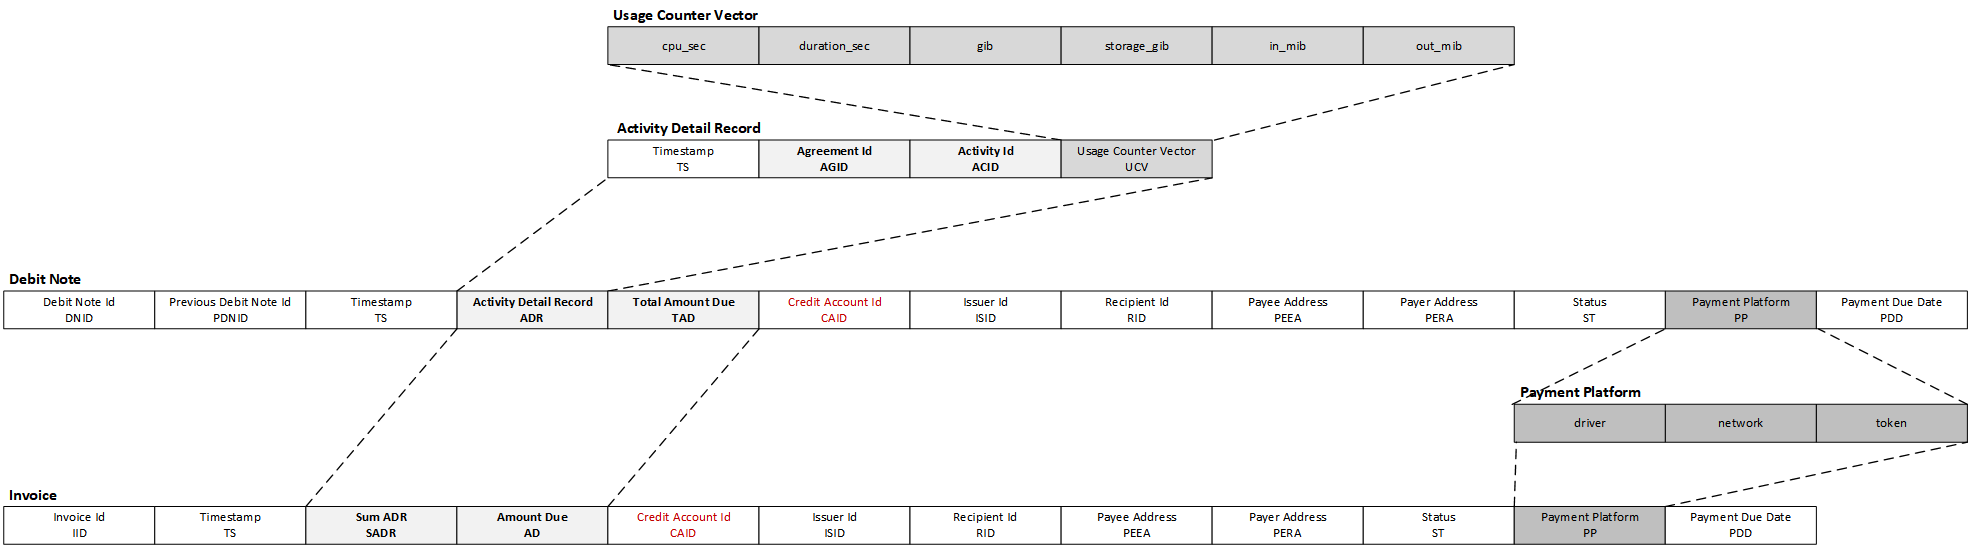
\includegraphics[width=17cm,angle=0]{./diag/Reference/PaymentFrame-1-Reference.png}
	\caption{Debit Note and Invoice Objects Frame}
    \label{fig:PF1}
\end{figure}

\begin{figure}[H]
    \centering
    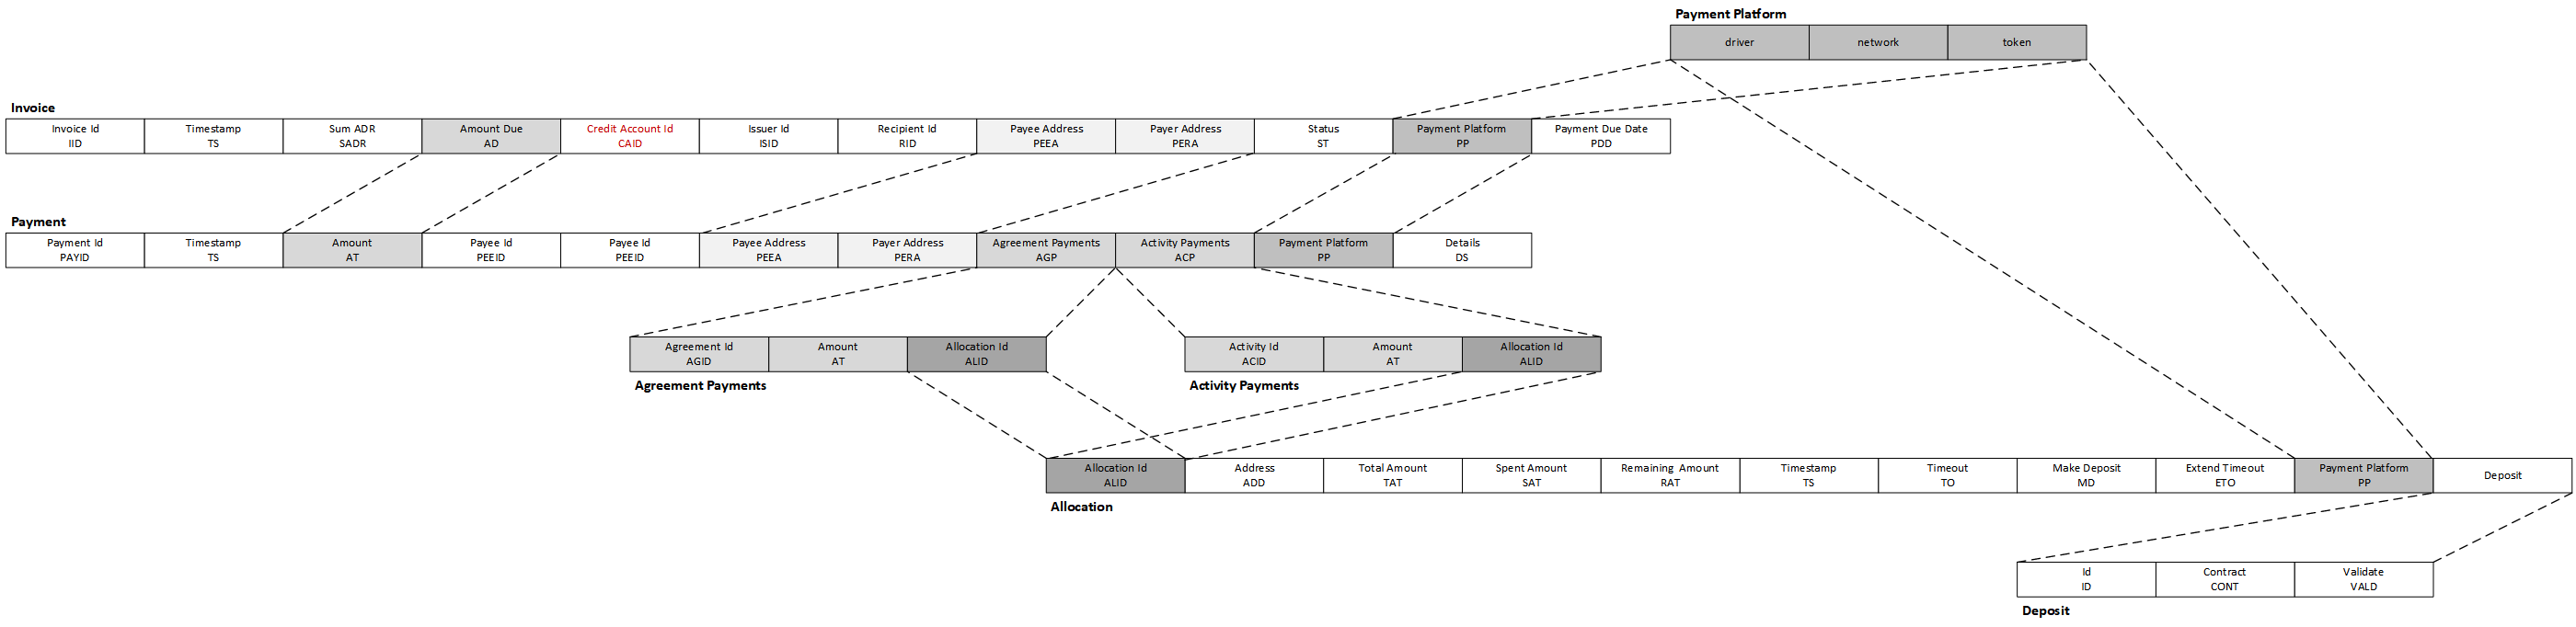
\includegraphics[width=19cm,angle=0]{./diag/Reference/PaymentFrame-2-Reference.png}
	\caption{Payment Objects Frame}
    \label{fig:PF2}
\end{figure}

\begin{enumerate}

\item Usage Counter Vector Objects

\begin{enumerate}

\item Object Description

TODO !!

\item Object Fields

\begin{table}[H]
\footnotesize

\begin{center}
\begin{tabular}{|p{3cm}|l|p{3cm}|p{3cm}|p{4cm}|} 
\hline
\rowcolor{lightgray}	Name	& MO.	& Type	& Example & 	Description \\
\hline

{\it counter} 	& O & string & cpu\_sec		& Counter \\
\hline 		

\end{tabular}
\end{center}
\end{table}

\item Object State

Stateless object

\end{enumerate}

\item Activity Detail Record

\begin{enumerate}

\item Object Description

TODO !!

\item Object Fields

\begin{table}[H]
\footnotesize

\begin{center}
\begin{tabular}{|p{3cm}|l|p{3cm}|p{3cm}|p{4cm}|} 
\hline
\rowcolor{lightgray}	Name	& MO.	& Type	& Example & 	Description \\
\hline

timestamp 			& M & string(\$date-time) 	&  YYYY-MM-DDThh:mm:ss.sssZ	&  \\
\hline

agreementId 		& M & string 				&  							&  Agreement Identifier \\
\hline	

activityId 			& M & string 				&  							&  Activity Identifier \\
\hline

usageCounterVector	& M & object				&							&  Usage Counter Vector \\
\hline

\end{tabular}
\end{center}
\end{table}

\item Object State

Stateless object

\end{enumerate}

\item Debit Note

\begin{enumerate}

\item Object Description

Debit Note is an object issued by Provider node to Requestor node, in the context of a specific Activity.
Activity Context is defined as a set of computational resource metrics, called Usage Counter Vector.
It is a notification of Total Amount Due incurred by the Activity until the Debit Note is issued.

%This is expected to be used as trigger for payment in upfront-payment or pay-as-you-go scenarios.

Debit Note can be used for payment in the scenario:

\begin{itemize}

\item upfront-payment

Payment in advance makes sense when the Agreement concerns multiple activities and 
the settlement concerns the time of resource lease and not its disposal.

\item pay-as-you-go

Payment with current usage makes sense when the activity on the resources is longer and partial payment terms 
are agreed with optimized transaction costs.

\end{itemize}

Debit Notes means the current Total Amount Due, which is calculated from the beginning of the Activity.
Debit Notes calculate the payment amount based on the difference between the Total Payments 
for the Agreement and the Total Amount Due.

\item Object Fields

\begin{table}[H]
\footnotesize

\begin{center}
\begin{tabular}{|p{3cm}|l|p{3cm}|p{3cm}|p{4cm}|} 
\hline
\rowcolor{lightgray}	Name	& MO.	& Type	& Example & 	Description \\
\hline

debitNoteId 			& M & string 				&  							&  Debit Note Identifier \\
\hline	

previousDebitNoteId 	& M & string 				&  							&  Last Debit Note Identifier \\
\hline	

timestamp 				& M & string(\$date-time) 	&  YYYY-MM-DDThh:mm:ss.sssZ	&  \\
\hline

ActivityDetailRecord	& M & object 				&  							&  Activity Detail Record \\
\hline	

totalAmountDue 			& M & string 				&  							&   \\
\hline

usageCounterVector		& M & object				&							&  Usage Counter Vector \\
\hline

issuerId				& M &  string				&							& Issuer Identifier \\
\hline

recipientId				& M & string 				&  							&   \\
\hline

payeeAddr				& M & string 				&  							&   \\
\hline

payerAddr				& M & string 				&  							&   \\
\hline

paymentPlatform			& M & string 				&  							&   \\
\hline

paymentDueDate			& M & string(\$date-time) 	&  YYYY-MM-DDThh:mm:ss.sssZ	&  \\
\hline

status					& M & string(enum)			& [ ISSUED, RECEIVED, ACCEPTED, REJECTED, FAILED, SETTLED, CANCELLED ] & Debit Note Status \\
\hline
			
\end{tabular}
\end{center}
\end{table}

\item Object State

(Please see Figure ~\ref{fig:DNSD} on page ~\pageref{fig:DNSD}).

\begin{figure}[H]
    \centering
    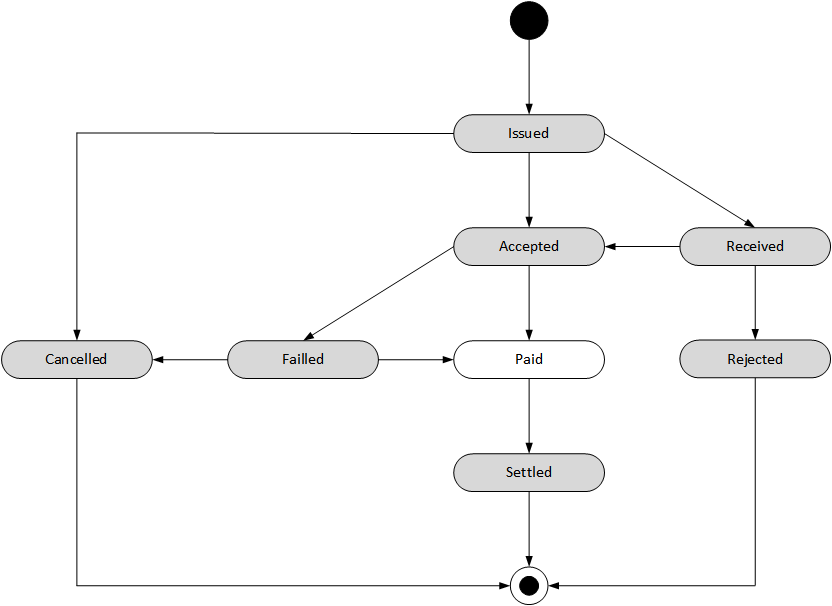
\includegraphics[width=9cm,angle=0]{./diag/Reference/DebitNoteState-Reference.png}
	\caption{Debit Note Status Diagram}
    \label{fig:DNSD}
\end{figure}

\begin{table}[H]
\footnotesize

\begin{center}
\begin{tabular}{|p{3cm}|p{11cm}|} 
\hline
\rowcolor{lightgray}	Status	& 	Description \\
\hline

Issued		&	 	\\
\hline
Received	&		\\
\hline
Accepted 	& 		\\
\hline
Rejected 	&		\\
\hline
Failed		&		\\
\hline
Settled		&		\\
\hline
Cancelled	&		\\
\hline
Paid		&	currently not implemented	\\
\hline

\end{tabular}
\end{center}
\end{table}

\end{enumerate}

\item Invoice

\begin{enumerate}

\item Object Description

The Invoice object is issued by the Provider node for the Requestor node,
in the context of a specific Agreement (Agreement object).
The context of the agreement is defined as a set of consents to the provision of a service and which was made within the Activity.
It indicates the total amount due from the Applicant under this Agreement.
After the Invoice is issued, no further Debit Notes will be issued.
Issuing an Invoice means Termination of the Agreement (if it has not already been terminated).
After the Invoice is issued, no Activities are allowed to be performed.


\item Object Fields

\begin{table}[H]
\footnotesize

\begin{center}
\begin{tabular}{|p{3cm}|l|p{3cm}|p{3cm}|p{4cm}|} 
\hline
\rowcolor{lightgray}	Name	& MO.	& Type	& Example & 	Description \\
\hline

invoiceId	 			& M & string 				&  							&  Debit Note Identifier \\
\hline	

timestamp 				& M & string(\$date-time) 	&  YYYY-MM-DDThh:mm:ss.sssZ	&  \\
\hline

agreementId				& M & string 				&  							&  Agreement Identifier \\
\hline	

activityIds				& O & string(list)			&							& List of activityIds \\
\hline

amount	 				& M & string 				&  							&   \\
\hline

issuerId				& M &  string				&							& Issuer Identifier \\
\hline

recipientId				& M & string 				&  							&   \\
\hline

payeeAddr				& M & string 				&  							&   \\
\hline

payerAddr				& M & string 				&  							&   \\
\hline

paymentPlatform			& M & object(json) 			&  							&   \\
\hline

paymentDueDate			& M & string(\$date-time) 	&  YYYY-MM-DDThh:mm:ss.sssZ	&  \\
\hline

status					& M & string(enum)			& [ ISSUED, RECEIVED, ACCEPTED, REJECTED, FAILED, SETTLED, CANCELLED ] & Invoice Status \\
\hline
			
\end{tabular}
\end{center}
\end{table}

\item Object State

(Please see Figure ~\ref{fig:ISD} on page ~\pageref{fig:ISD}).

\begin{figure}[H]
    \centering
    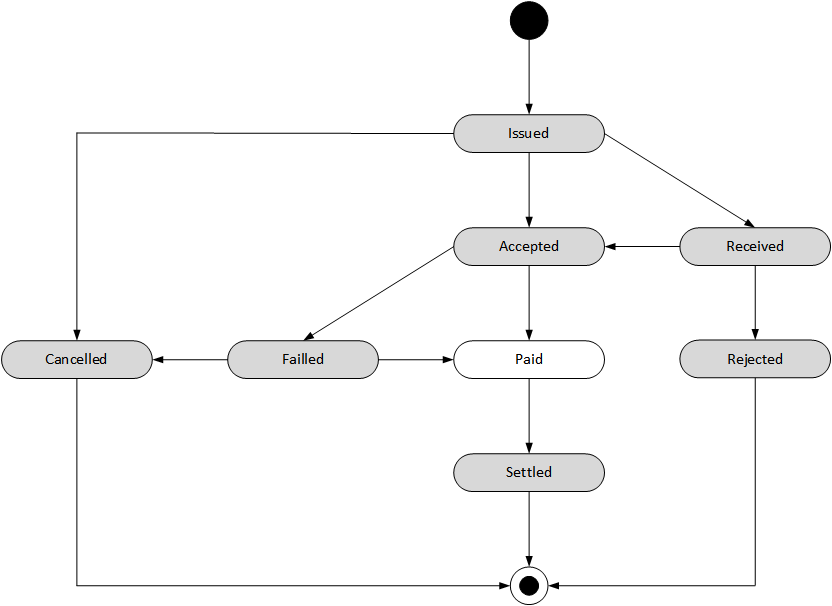
\includegraphics[width=9cm,angle=0]{./diag/Reference/InvoiceState-Reference.png}
	\caption{Invoice Status Diagram}
    \label{fig:ISD}
\end{figure}

\begin{table}[H]
\footnotesize

\begin{center}
\begin{tabular}{|p{3cm}|p{11cm}|} 
\hline
\rowcolor{lightgray}	Status	& 	Description \\
\hline

Issued		&	 	\\
\hline
Received	&		\\
\hline
Accepted 	& 		\\
\hline
Rejected 	&		\\
\hline
Failed		&		\\
\hline
Settled		&		\\
\hline
Cancelled	&		\\
\hline
Paid		&	currently not implemented	\\
\hline

\end{tabular}
\end{center}
\end{table}

\end{enumerate}


\item PaymentPlatform Object

\begin{enumerate}

\item Object Description

PaymentPlatform is a object that is helping to chose which driver and network to use

\item Object Fields

\begin{table}[H]
\footnotesize

\begin{center}
\begin{tabular}{|p{3cm}|l|p{3cm}|p{3cm}|p{4cm}|} 
\hline
\rowcolor{lightgray}	Name	& MO.	& Type	& Example & 	Description \\
\hline

driver		& O & string				&							& 							\\
\hline
network		& O & string				&							& 							\\
\hline
token		& O & string				&							& 							\\
\hline

\end{tabular}
\end{center}
\end{table}

\item Object State

Stateless object

\end{enumerate}

% Allocation

\item Allocation Object

\begin{enumerate}

\item Object Description

An Allocation is a designated sum of money reserved for the purpose of making some particular payments. 
Allocations are currently purely virtual objects. 
They exist only in Requestor's database. 
An Allocation is connected to a payment account (wallet) specified by address and paymentPlatform field. 
If these fields are not present the default payment platform is used and the address is assumed to be 
identical to the Requestor's Node ID.

\item Object Fields

\begin{table}[H]
\footnotesize

\begin{center}
\begin{tabular}{|p{3cm}|l|p{3cm}|p{3cm}|p{4cm}|} 
\hline
\rowcolor{lightgray}	Name	& MO.	& Type	& Example & 	Description \\
\hline

allocationId			& M & string 				&							&  \\
\hline

address					& O & string 				&							&  \\
\hline

paymentPlatform			& O & object(json)			&							&	\\
\hline

totalAmount				& M & string 				&							&  \\
\hline

spentAmount				& M & string 				&							&  \\
\hline

remainingAmount			& M & string 				&							&  \\
\hline

timestamp 				& M & string(\$date-time) 	&  YYYY-MM-DDThh:mm:ss.sssZ	&  \\
\hline

timeout					& O & string(\$date-time) ?? &							&  \\
\hline

makeDeposit				& O & boolean				&							&  \\
\hline

extendTimeout			& O & integer(\$int64)		&							& 	in seconds, the time by which the allocation timeout is extended 
																					after it is last used. \\
\hline

deposit.id				& M & string 				&							&  \\
\hline

deposit.contract		& M & string 				&							&  \\
\hline

deposit.validate		& O & json					& 							& 	\\
\hline
			
\end{tabular}
\end{center}
\end{table}

\item Object State

Stateless object

\end{enumerate}

\item AgreementPayment Object

\begin{enumerate}

\item Object Description

Share of a Payment assigned to an Agreement, but not to any particular Activity within that Agreement.

\item Object Fields

\begin{table}[H]
\footnotesize

\begin{center}
\begin{tabular}{|p{3cm}|l|p{3cm}|p{3cm}|p{4cm}|} 
\hline
\rowcolor{lightgray}	Name	& MO.	& Type	& Example & 	Description \\
\hline

agreementId		& M & string				&							& 							\\
\hline

amount			& M & string				&							& 							\\
\hline

allocationId	& O & string				&							& 							\\
\hline

\end{tabular}
\end{center}
\end{table}

\item Object State

Stateless object

\end{enumerate}

\item ActivityPayment Object

\begin{enumerate}

\item Object Description

Share of a Payment assigned to a particular Activity.

\item Object Fields

\begin{table}[H]
\footnotesize

\begin{center}
\begin{tabular}{|p{3cm}|l|p{3cm}|p{3cm}|p{4cm}|} 
\hline
\rowcolor{lightgray}	Name	& MO.	& Type	& Example & 	Description \\
\hline

activityId		& M & string				&							& 							\\
\hline

amount			& M & string				&							& 							\\
\hline

allocationId	& O & string				&							& 							\\
\hline

\end{tabular}
\end{center}
\end{table}

\item Object State

Stateless object

\end{enumerate}

\item Payment Object

\begin{enumerate}

\item Object Description

A Payment is a single transaction sent from Requestor to Provider. 
A single payment can be made for multiple Agreements and Activities. 
AgreementPayments and ActivityPayments specify what is the basis for payment.

\item Object Fields

\begin{table}[H]
\footnotesize

\begin{center}
\begin{tabular}{|p{3cm}|l|p{3cm}|p{3cm}|p{4cm}|} 
\hline
\rowcolor{lightgray}	Name	& MO.	& Type	& Example & 	Description \\
\hline

paymentId			& M & string				&							&							\\
\hline

payerId				& M & string				&							&							\\
\hline

payeeId				& M & string				&							&							\\
\hline

payerAddr			& M & string				&							&							\\
\hline

payeeAddr			& M & string				&							&							\\
\hline

paymentPlatform		& M & string				&							&							\\
\hline

amount				& M & string				&							&							\\
\hline

timestamp			& M & string(\$date-time)	&							&							\\
\hline

agreementPayments	& M & object(json)			&							&							\\
\hline

activityPayments	& M & object(json)			&							&							\\
\hline
	
details				& M & string(\$byte)		&							&							\\
\hline

\end{tabular}
\end{center}
\end{table}

\item Object State

Stateless object

\end{enumerate}

\end{enumerate}

%%%% Payment Operations TODO

The Payment Space is used to define interaction operations on these objects such as:

\begin{enumerate}


\item  Rating Operation

\begin{enumerate}

\item Description

The Rating operation is implemented by a set of functions with REST API methods that allow you to transform measurement 
data into debit note items (Debit Note object) based on the agreed price plan.

The IssueDebitNote() function is used to create a debit note based on the Activity Detail Record object (ADR object).
This object collects measurement data from the Usage Counter Vector (UCV) object of the service in a time interval.
This data is associated with the activity (activityId) and the agreement (agreementId). This function is initialized on the Provider node.
Using the REST /send method allows you to send the created Debit Note object from the Provider node to the Requestor node.
The CollectDebitNoteInvoiceEvent() function is used to collect debit notes and their states from the network.
It listens for events related to the debit note using long polling.
If there are any events, the method associated with the function (/debitNoteEvents) will return them immediately.
If there are none, the method will wait until at least one event occurs or the timeout expires.
The afterTimestamp parameter can be used to get only "new" events.
Setting the parameter value to the timestamp of the last processed event ensures that no event is missed.
The events are persistent, i.e. the API call does not remove event records from the receiving queue.
The AcceptDebitNote() function is used to signal the acceptance of a received debit note by the Requestor node.
The acceptance event is sent to the network. And via the CollectDebitNoteInvoiceEvent() function, this event is collected
by the Provider node.
The CancelDebitNote() function is used to signal the cancellation of a generated debit note by the Provider node.
The RejectDebitNote() function is used to signal the rejection of a received debit note by the Requestor node.
From both nodes, you can call the REST methods /debitNotes and /debitNotes/\{debitNoteId\} to retrieve information about
debit notes.

(Please see Figure ~\ref{fig:RO} on page ~\pageref{fig:RO}).

\item Sequence Diagram

\begin{figure}[H]
    \centering
    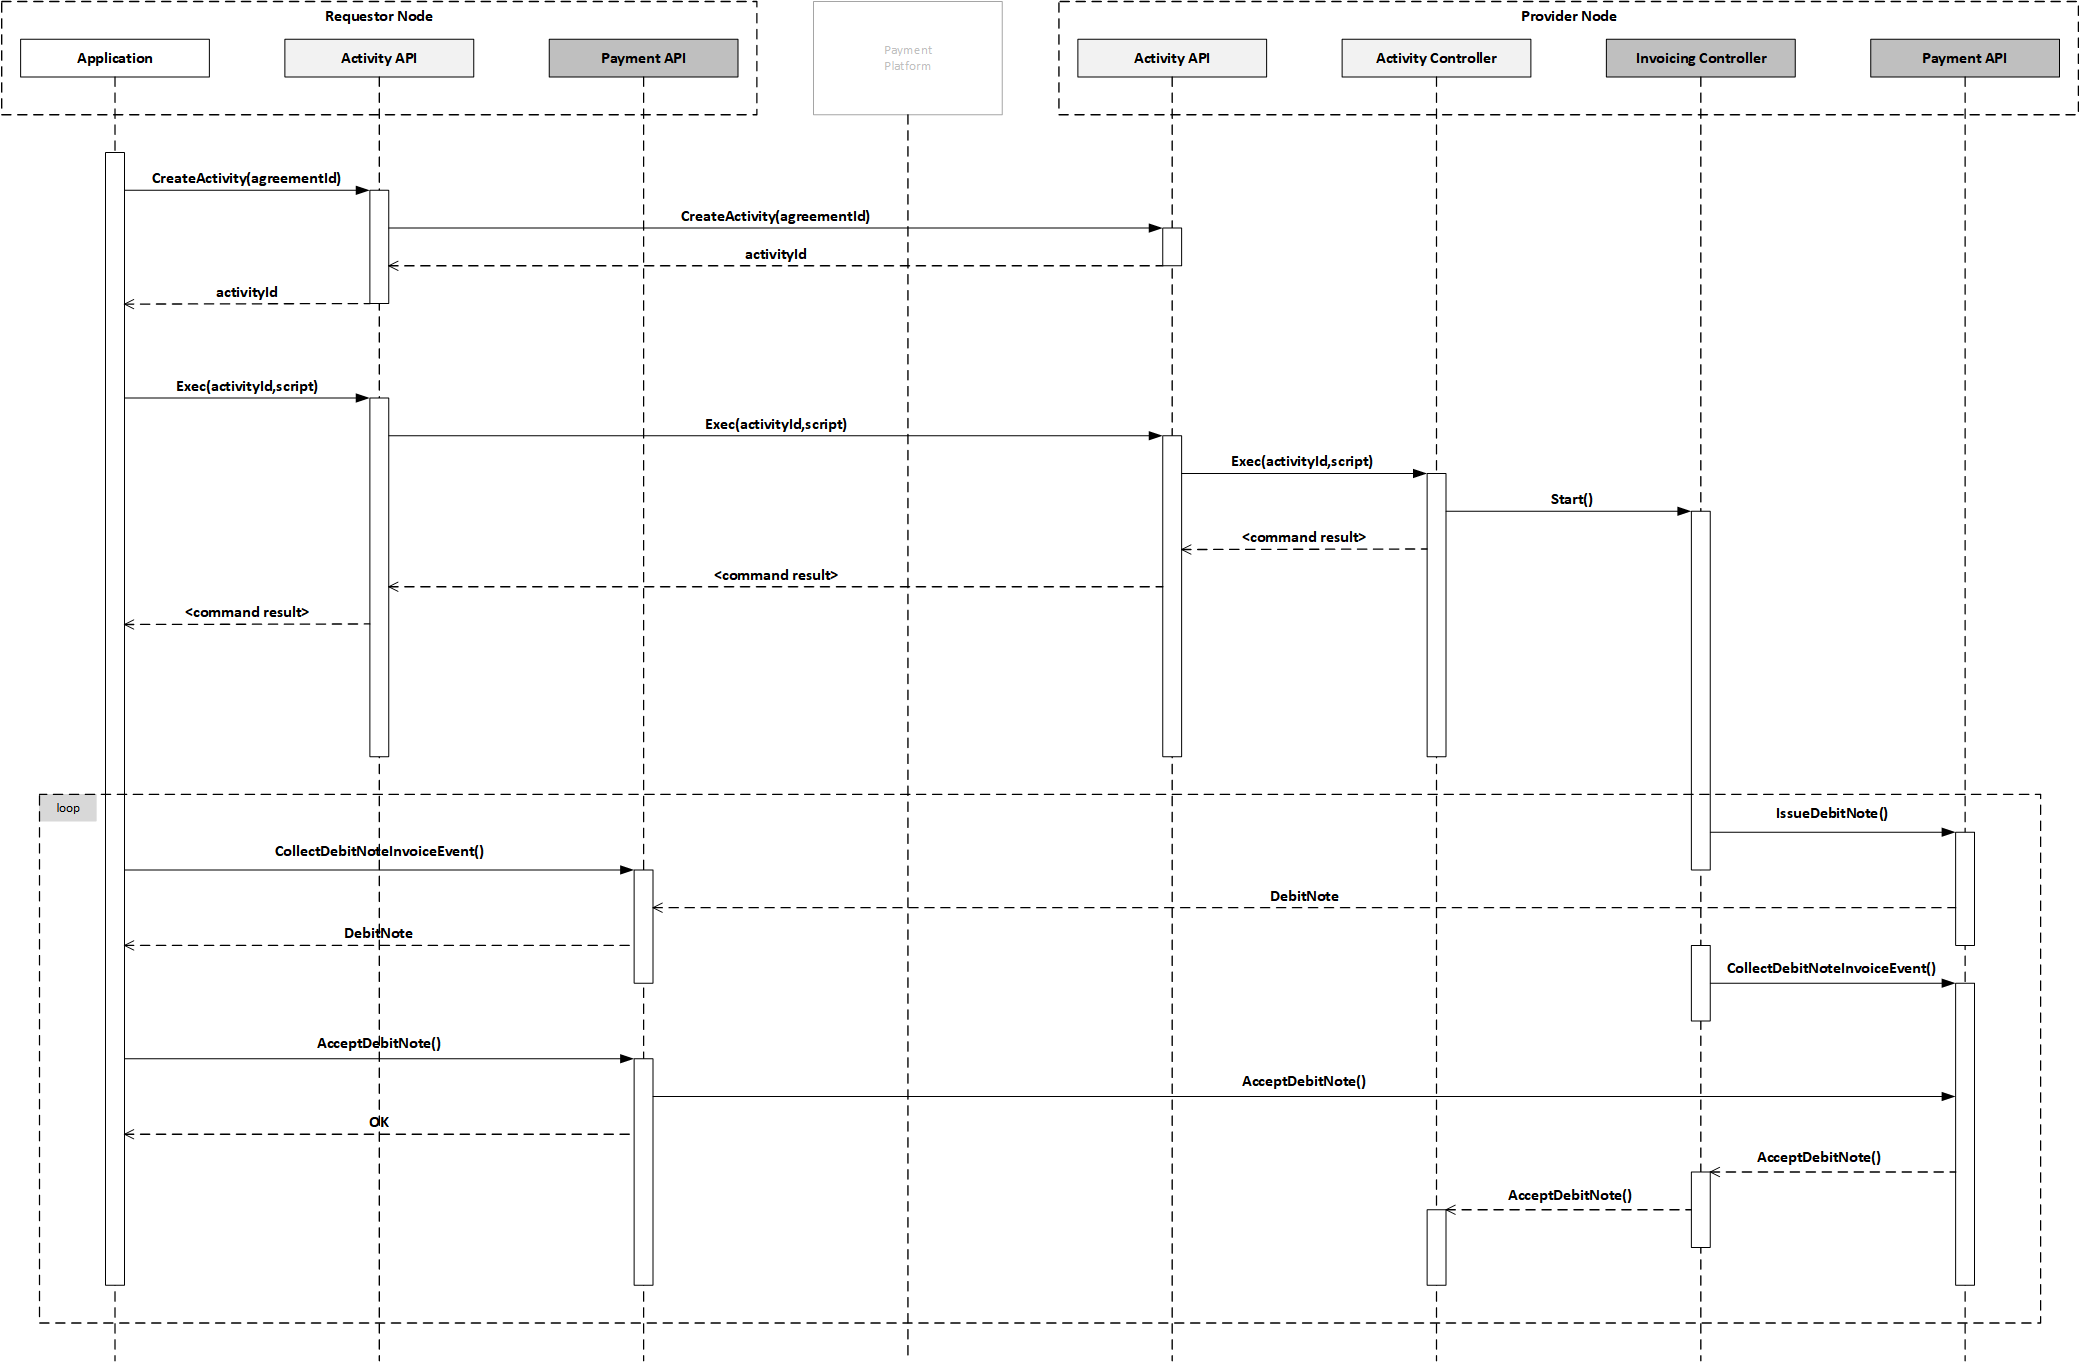
\includegraphics[width=18cm,angle=0]{./diag/Sequence/PaymentRating-B-Sequence.png}
	\caption{Rating Operation}
    \label{fig:RO}
\end{figure}

\item Functions and Methods

\begin{table}[H]
\footnotesize

\begin{center}
\begin{tabular}{|p{3cm}|p{7cm}|p{1.5cm}|p{4cm}|} 
\hline
\rowcolor{lightgray}	Function Name	& API Method Name				& 	Side		&	Description \\
\hline

IssueDebitNote			&	POST /debitNotes							& 	Provider	&	Issue a Debit Note	\\
\hline

						& 	POST /debitNotes/\{debitNoteId\} /send		&	Provider 	&	Send Debit Note to Requestor \\
\hline

CancelDebitNote			&	POST /debitNotes/\{debitNoteId\} /cancel	&	Provider	&	Cancel Debit Note \\
\hline

CollectDebitNote \newline InvoiceEvent	&	GET /debitNoteEvents		&	Both		&	Get Debit Note events \\
\hline

AcceptDebitNote			&	POST /debitNotes/\{debitNoteId\} /accept	&	Requestor	&	Accept received Debit Note \\
\hline

						& 	GET /debitNotes								&	Both		& 	List Debit Notes \\
\hline

						& 	GET /debitNotes/\{debitNoteId\}				&	Both 		&	Get Debit Note \\
\hline

RejectDebitNote			&	POST /debitNotes/\{debitNoteId\} /reject	&	Requestor	&	Reject received Debit Note \\
\hline

RejectionReasion		&												&	Requestor	&	{\it Unsolicited service} 
																							\newline 	{\it Bad Service}
																							\newline 	{\it Incorrect Amount} \\
\hline
						
\end{tabular}
\end{center}
\end{table}

\end{enumerate}

\item  Billing Operation

\begin{enumerate}

\item Description

The Billing operation consists of functions with REST API methods that are used to implement the process of issuing invoices 
based on the use of the service according to the agreed price plan.

The IssueInvoice() function is used to create and send an invoice (Invoice object) from the Provider node to the Requestor node
in the context of a specific Agreement.
It indicates the total amount due from the Applicant under this Agreement.
After issuing an Invoice, no further Debit Notes will be issued.
Issuing an Invoice means Terminating the Agreement (if it has not already been terminated).
After issuing an Invoice, no Actions are allowed.
The CollectDebitNoteInvoiceEvent() function is used to collect invoices and their states from the network.
It listens for debit note events using long polling.
If there are any events, the method associated with the function (/invoicesEvents) will return them immediately.
If there are none, the method will wait until at least one event occurs or the timeout expires.
The afterTimestamp parameter can be used to get only "new" events.
Setting the parameter value to the timestamp of the last processed event ensures that no event goes unnoticed.
The events are persistent, i.e. the API call does not remove event records from the receiving queue.
The AcceptInvoice() unction is used to signal the acceptance of the received invoice by the Requestor node.
The acceptance event is sent to the network. And via the CollectDebitNoteInvoiceEvent() function, this event is collected
by the Provider node.
The CancelInvoice() function is used to signal the cancellation of the generated invoice by the Provider node.
The RejectInvoice() function is used to signal the rejection of the received invoice by the Requestor node.
From both nodes you can call the REST methods /invoices and /invoices/\{invoiceId\} to retrieve information about invoices.

(Please see Figure ~\ref{fig:BO} on page ~\pageref{fig:BO}).

\item Sequence Diagram

\begin{figure}[H]
    \centering
    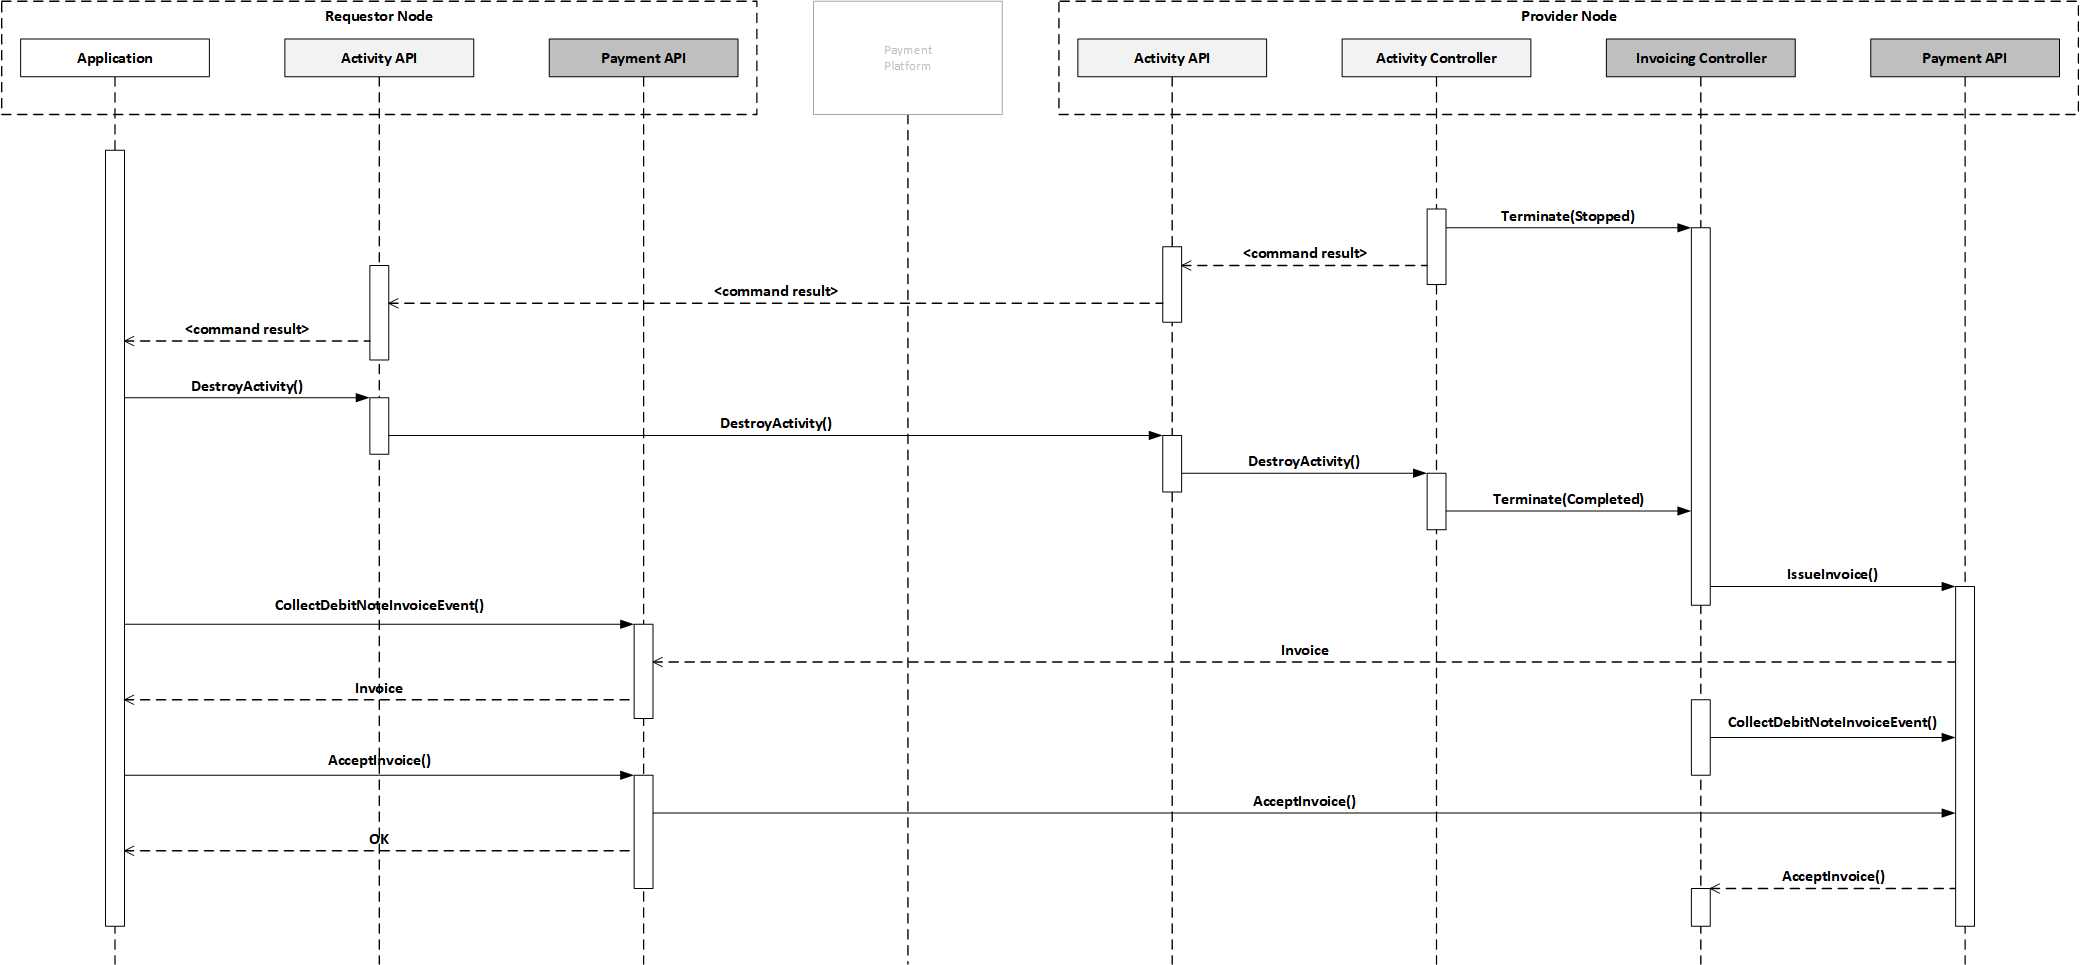
\includegraphics[width=18cm,angle=0]{./diag/Sequence/PaymentBilling-B-Sequence.png}
	\caption{Billing Operation}
    \label{fig:BO}
\end{figure}

\item Functions and Methods

\begin{table}[H]
\footnotesize

\begin{center}
\begin{tabular}{|p{3cm}|p{7cm}|p{1.5cm}|p{4cm}|} 
\hline
\rowcolor{lightgray}	Function Name	& API Method Name				& 	Side		&	Description \\
\hline

IssueInvoice			&	POST /invoices								&	Provider	&	Issue an Invoice \\
\hline

AcceptInvoice			&	POST /invoices/\{invoiceId\} /accept		&	Requestor 	&	Accept received Invoice \\
\hline

RejectInvoice			&	POST /invoices/\{invoiceId\} /reject		&	Requestor 	&	Reject received Invoice \\
\hline

						& 	GET /invoices 								&	Both		&	List Invoices \\
\hline

						&	GET /invoices/\{invoiceId\}					&	Both		& 	Get Invoice \\
\hline

						&	POST /invoices/\{invoiceId\} /send			&	Provider 	& 	Send Invoice to Requestor \\
\hline 

						&	POST /invoices/\{invoiceId\} /cancel		&	Provider 	& 	Cancel Invoice  \\
\hline

						&	GET /invoiceEvents							&	Both 		& 	Get Invoice events \\
\hline

RejectionReasion		&												&	Requestor	&	{\it Unsolicited service} 
																							\newline 	{\it Bad Service}
																							\newline 	{\it Incorrect Amount} \\
\hline
						
\end{tabular}
\end{center}
\end{table}

\end{enumerate}


%%%% PAYMENT

\item Payment Operation

\begin{enumerate}

\item Description

The Payment operation consists of functions along with REST API methods that serve to implement 
the process of collecting the necessary information to make a payment for the service through 
the appropriate payment operator.

(Please see Figure ~\ref{fig:PO} on page ~\pageref{fig:PO}).

\item Sequence Diagram

\begin{figure}[H]
    \centering
    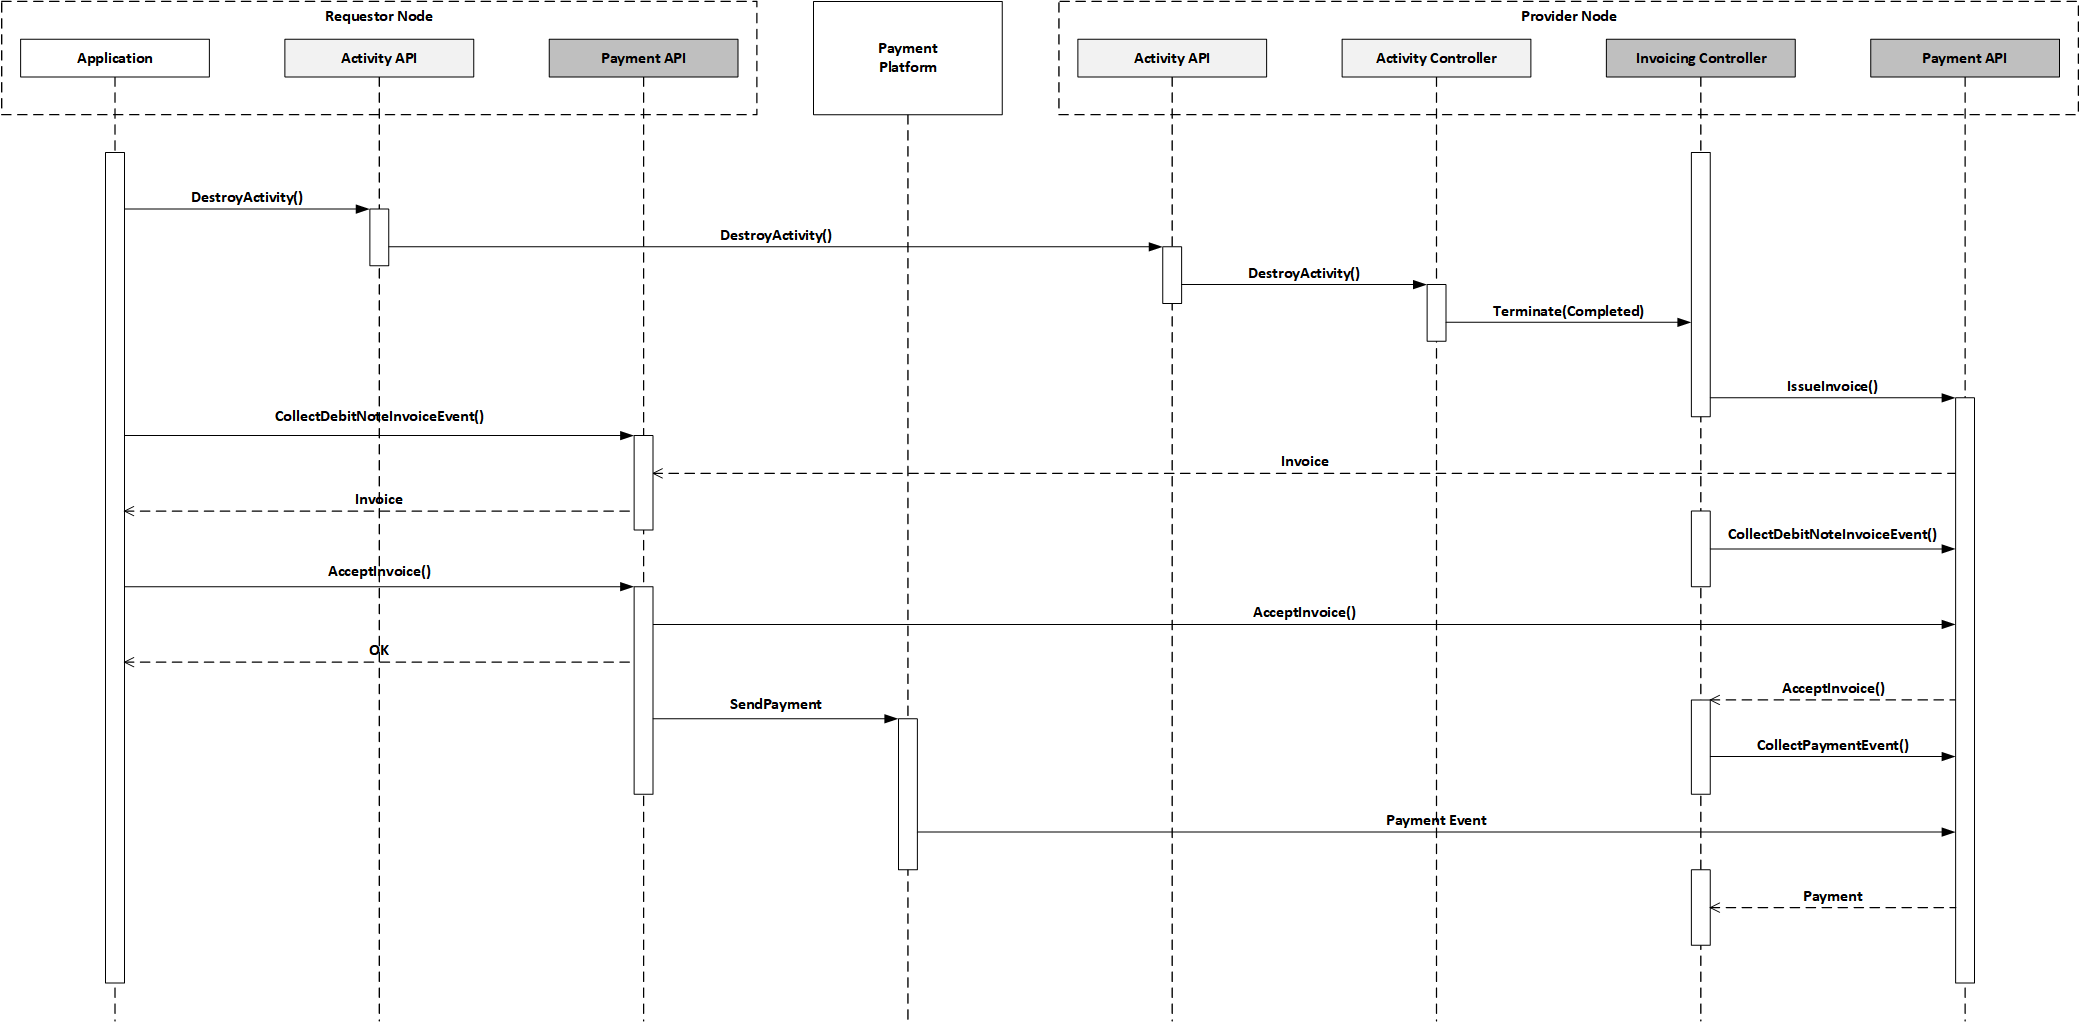
\includegraphics[width=18cm,angle=0]{./diag/Sequence/PaymentPayment-B-Sequence.png}
	\caption{Payment Operation}
    \label{fig:PO}
\end{figure}

\item Functions and Methods

\begin{table}[H]
\footnotesize

\begin{center}
\begin{tabular}{|p{3cm}|p{7cm}|p{1.5cm}|p{4cm}|} 
\hline
\rowcolor{lightgray}	Function Name	& API Method Name				& 	Side		&	Description \\
\hline

AllocateAmount			&	POST /allocations							&	Requestor 	&	Create Allocation \\
\hline

ListAllocations			&	GET /allocations 							&	Both		&	Get Allocations	\\
\hline

GetAllocationDetails	&	GET /allocations/\{allocationId\} 			&	Both		&	Get Allocation	\\
\hline

ReleaseAllocation		&	DELETE /allocations/\{allocationId\} 		&	Both		&	Release Allocation	\\
\hline

AmendAllocation			&	PUT /allocations/\{allocationId\} 			&	Both		&	Amend Allocation	\\
\hline

						&	GET /payments 								&	Both 		& 	Get payments \\
\hline

GetPaymentDetail		&	GET /payments/\{paymentId\}					&	Both 		&	Get payment \\
\hline

						& 	GET /payments/status 						& 	Both 		& 	Get status of the payment driver \\
\hline

CollectPaymentEvent		&												&	Provider 	&	Function used by Application process to 
																							collect notification of Payments arriving from PaymentPlatform \\
\hline

GetPayment ForDebitNote	&												&	Provider 	&	Function called by Provider to
																							obtain DebitNote-Payment mapping
																							required for payment reconciliation \\
\hline

GetPayment ForInvoice	&												&	Provider 	&	Function called by Provider to
																							obtain Invoice-Payment mapping
																							required for payment reconciliation \\
\hline

GetDemand Decorations	&	GET /demandDecorations 						&	Requestor	&	Function to extract the Demand (properties/constraints) specific to
																							a payment platform, which are necessary to place 
																							a payment-platform compliant Demand on the market \\
\hline

GetOffer Decorations	&						 						&	Provider	&	Function to extract the Offer (properties/constraints) specific to
																							a payment platform, which are necessary to place 
																							a payment-platform compliant Offer on the market \\
\hline
																									
						&	GET /providerAccounts						&	Provider 	&	Get available accounts for receiving payments \\
\hline

						&	GET /requestorAccounts						&	Requestor 	&	Get available accounts for receiving payments \\
\hline

GetSendAccounts			&												&	Requestor 	&	Function used by Application process on Requestor side to
																							list Accounts defined in the Daemon for the purpose of maiking payments. \\
\hline

GetReceiveAccounts		&												&	Provider 	&	Function used by Application process on Provider side to
																							list Accounts defined in the Daemon for the purpose of maiking payments. \\
\hline


\end{tabular}
\end{center}
\end{table}

\end{enumerate}

\end{enumerate}

\subsection{Golem Node Agent}

\subsubsection{User Application}

\begin{enumerate}

\item Provider

\item Requestor

\end{enumerate}

